\documentclass[11pt]{article}
\usepackage[textwidth=18.0cm, textheight=23.0cm, top=2.0cm]{geometry}
\usepackage{pst-all}
\usepackage{amssymb}
\usepackage{tikz}
\usepackage{underscore}\begin{document}
\pagestyle{empty}


ClassName: \underline{\textbf{Class_08.2bp-39}}
\par
BinSize: \underline{\textbf{100 × 100}}
\par
ReduceSize: \underline{\textbf{100 × 100}}
\par
TypeNum: \underline{\textbf{79}}
\par
Num: \underline{\textbf{80}}
\par
OutS: \underline{\textbf{240000}}
\par
InS: \underline{\textbf{208285}}
\par
Rate: \underline{\textbf{0.868}}
\par
UB: \underline{\textbf{24}}
\par
LB0: \underline{\textbf{24}}
\par
LB: \underline{\textbf{24}}
\par
LBWithCut: \underline{\textbf{24}}
\par
NodeCut: \underline{\textbf{0}}
\par
ExtendedNodeCnt: \underline{\textbf{1}}
\par
GenNodeCnt: \underline{\textbf{1}}
\par
PrimalNode: \underline{\textbf{0}}
\par
ColumnCount: \underline{\textbf{24}}
\par
TotalCutCount: \underline{\textbf{0}}
\par
RootCutCount: \underline{\textbf{0}}
\par
LPSolverCnt: \underline{\textbf{1}}
\par
PricingSolverCnt: \underline{\textbf{0}}
\par
BranchAndBoundNum: \underline{\textbf{1}}
\par
isOpt: \underline{\textbf{true}}
\par
TimeOnInitSolution: \underline{\textbf{2.690 s}}
\par
TimeOnPrimal: \underline{\textbf{0.000 s}}
\par
TimeOnPricing: \underline{\textbf{0.000 s}}
\par
TimeOnRmp: \underline{\textbf{0.062 s}}
\par
TotalTime: \underline{\textbf{2.815 s}}
\par
\newpage


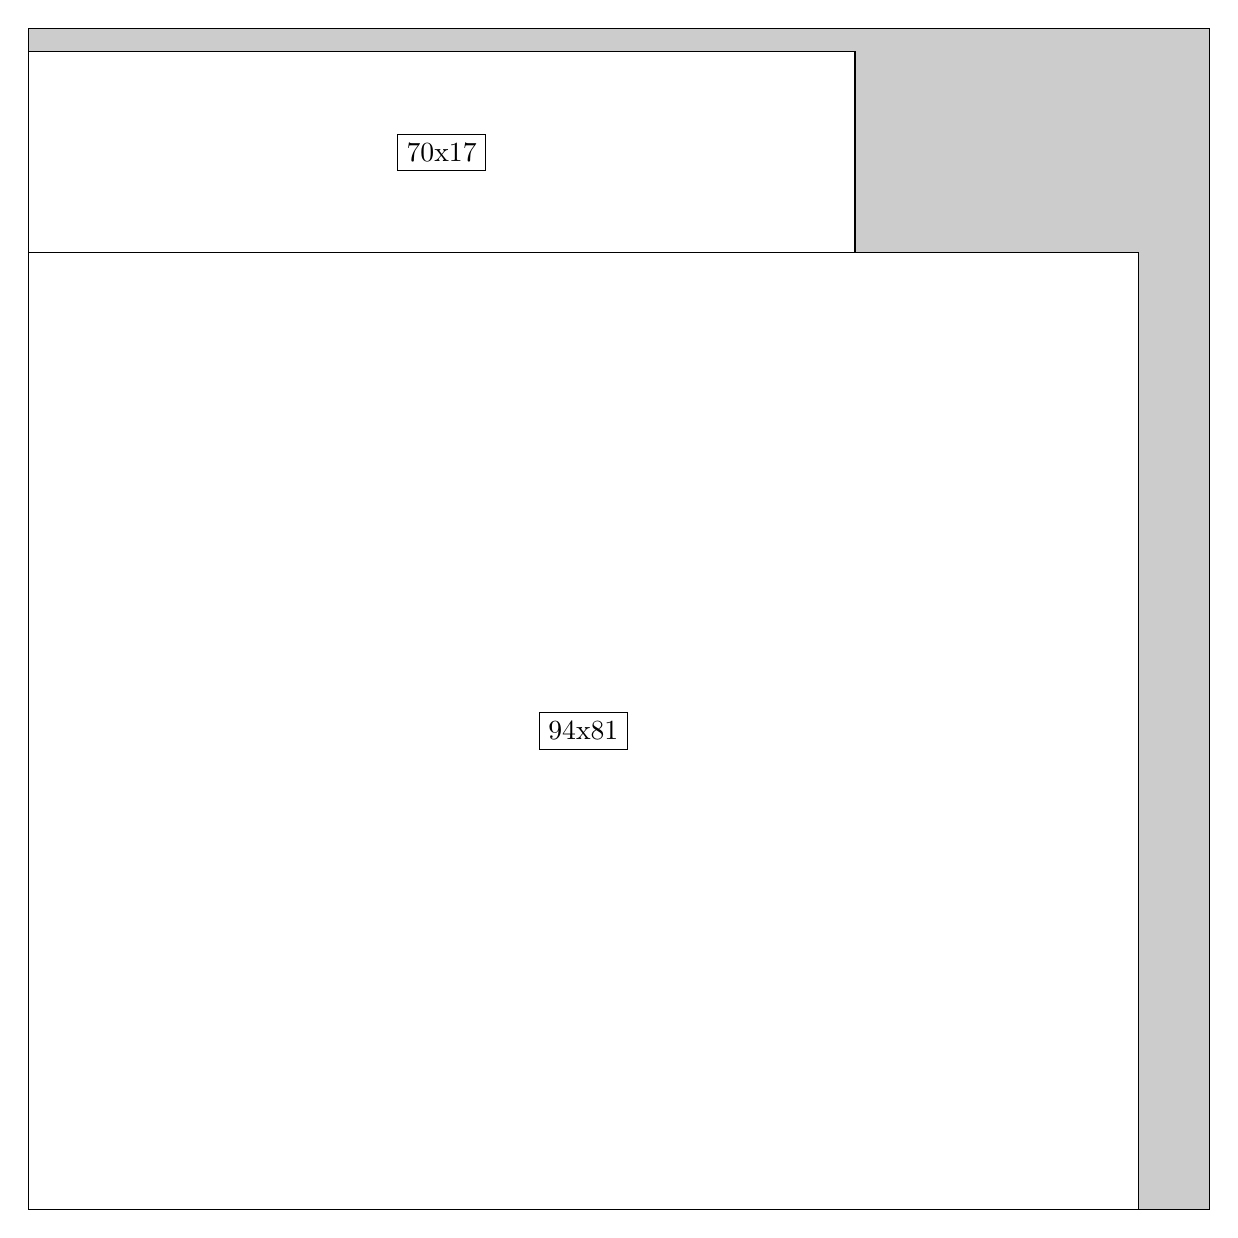
\begin{tikzpicture}[shorten >=1pt,scale=1.0,every node/.style={scale=1.0},->]
\tikzstyle{vertex}=[circle,fill=black!25,minimum size=14pt,inner sep=0pt]
\filldraw[fill=gray!40!white, draw=black] (0,0) rectangle (15.0,15.0);
\foreach \name/\x/\y/\w/\h in {94x81/0.0/0.0/14.1/12.15,70x17/0.0/12.15/10.5/2.55}
\filldraw[fill=white!40!white, draw=black] (\x,\y) rectangle node[draw] (\name) {\name} ++(\w,\h);
\end{tikzpicture}


w =94 , h =81 , x =0 , y =0 , v =7614
\par
w =70 , h =17 , x =0 , y =81 , v =1190
\par
\newpage


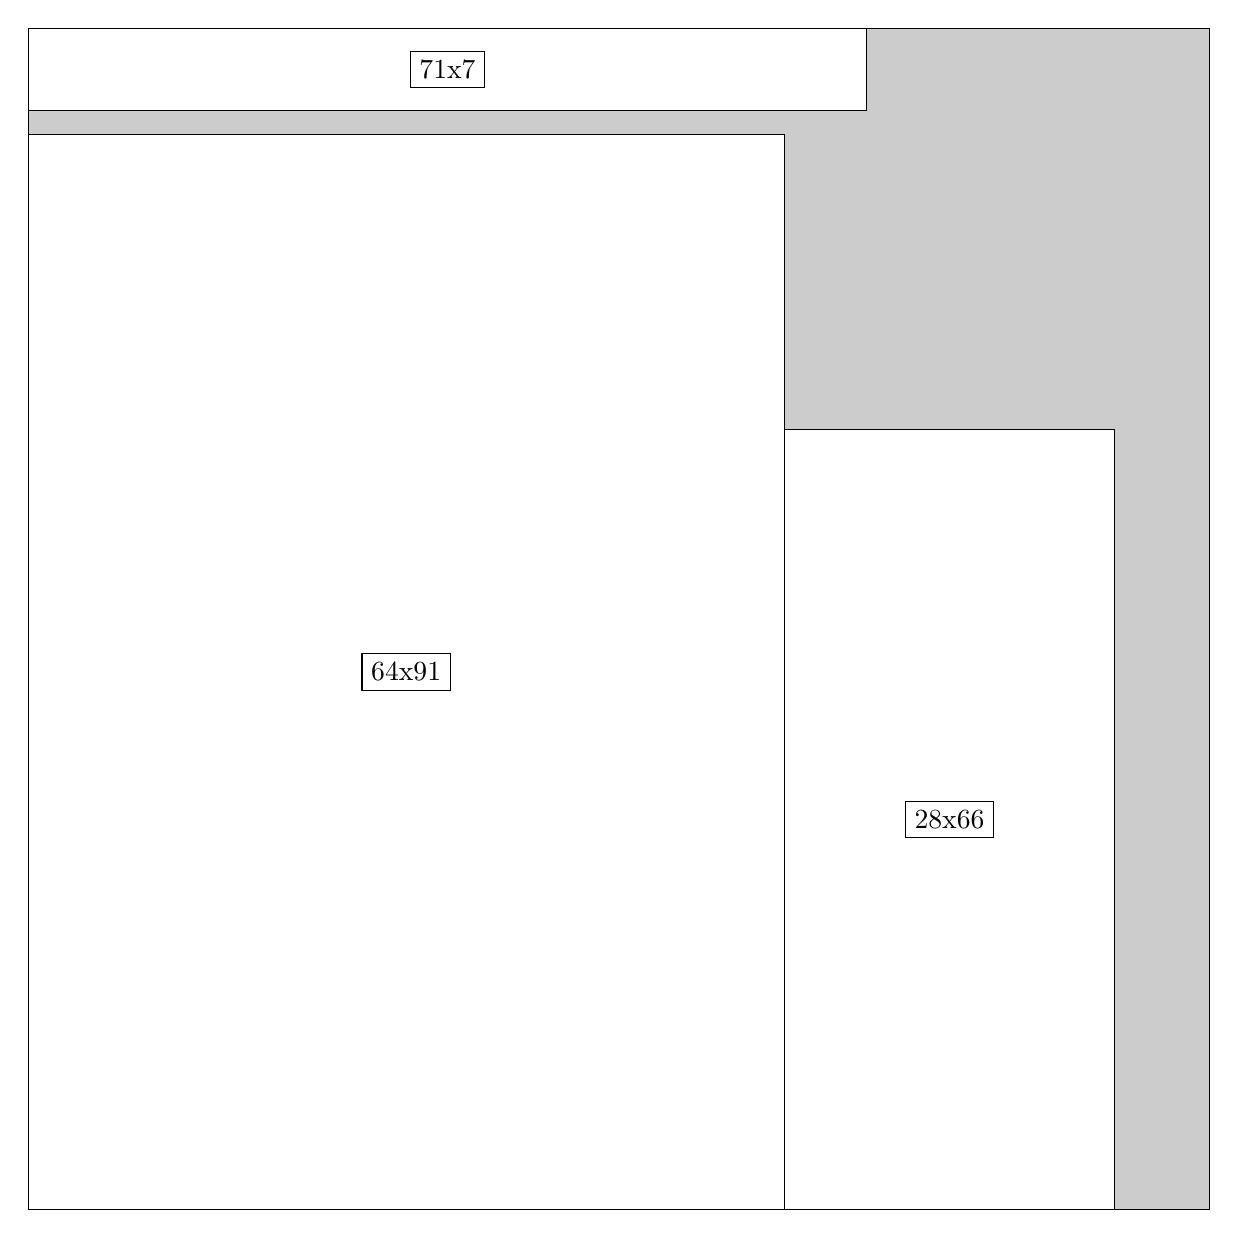
\begin{tikzpicture}[shorten >=1pt,scale=1.0,every node/.style={scale=1.0},->]
\tikzstyle{vertex}=[circle,fill=black!25,minimum size=14pt,inner sep=0pt]
\filldraw[fill=gray!40!white, draw=black] (0,0) rectangle (15.0,15.0);
\foreach \name/\x/\y/\w/\h in {64x91/0.0/0.0/9.6/13.65,28x66/9.6/0.0/4.2/9.9,71x7/0.0/13.95/10.65/1.05}
\filldraw[fill=white!40!white, draw=black] (\x,\y) rectangle node[draw] (\name) {\name} ++(\w,\h);
\end{tikzpicture}


w =64 , h =91 , x =0 , y =0 , v =5824
\par
w =28 , h =66 , x =64 , y =0 , v =1848
\par
w =71 , h =7 , x =0 , y =93 , v =497
\par
\newpage


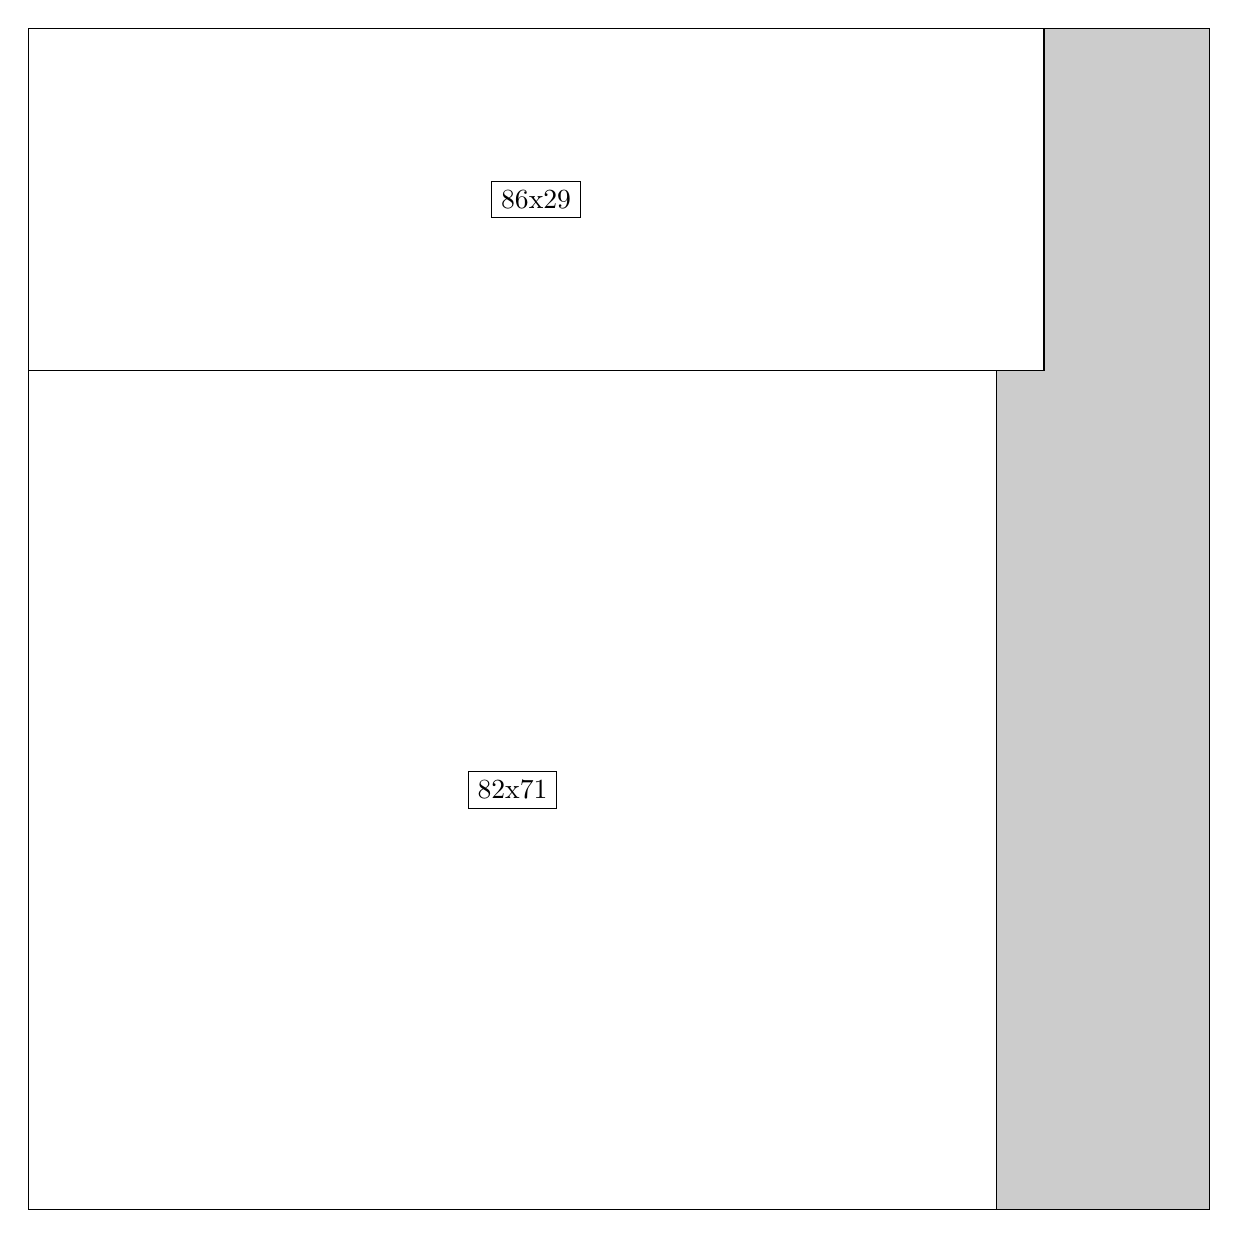
\begin{tikzpicture}[shorten >=1pt,scale=1.0,every node/.style={scale=1.0},->]
\tikzstyle{vertex}=[circle,fill=black!25,minimum size=14pt,inner sep=0pt]
\filldraw[fill=gray!40!white, draw=black] (0,0) rectangle (15.0,15.0);
\foreach \name/\x/\y/\w/\h in {82x71/0.0/0.0/12.299999999999999/10.65,86x29/0.0/10.65/12.9/4.35}
\filldraw[fill=white!40!white, draw=black] (\x,\y) rectangle node[draw] (\name) {\name} ++(\w,\h);
\end{tikzpicture}


w =82 , h =71 , x =0 , y =0 , v =5822
\par
w =86 , h =29 , x =0 , y =71 , v =2494
\par
\newpage


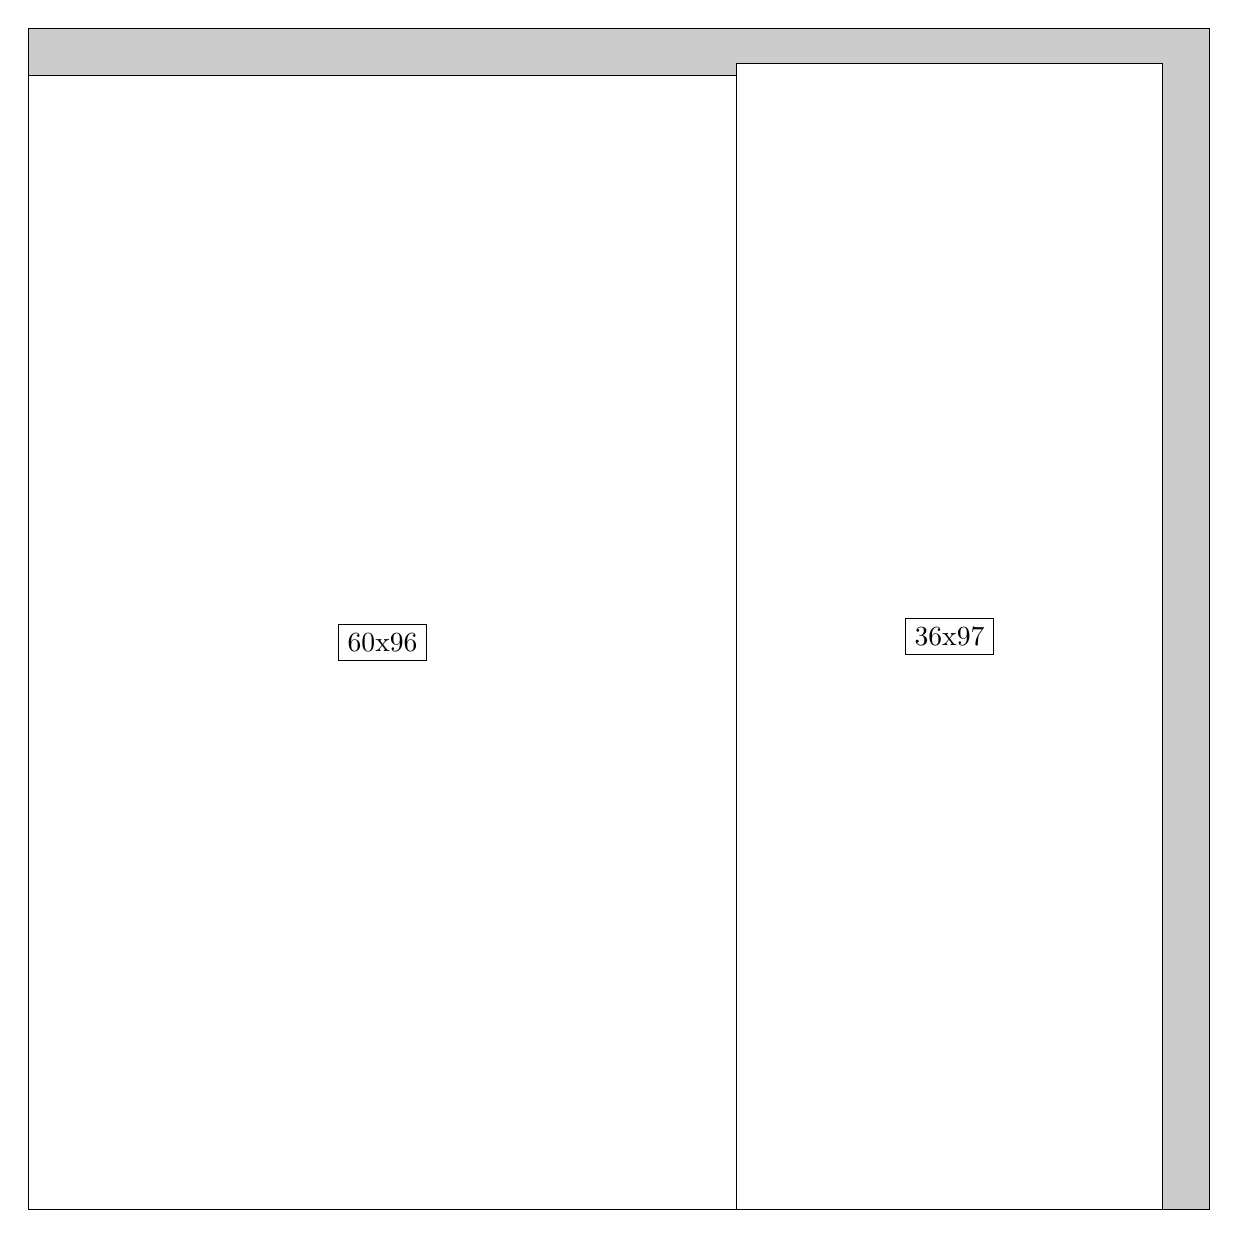
\begin{tikzpicture}[shorten >=1pt,scale=1.0,every node/.style={scale=1.0},->]
\tikzstyle{vertex}=[circle,fill=black!25,minimum size=14pt,inner sep=0pt]
\filldraw[fill=gray!40!white, draw=black] (0,0) rectangle (15.0,15.0);
\foreach \name/\x/\y/\w/\h in {36x97/9.0/0.0/5.3999999999999995/14.549999999999999,60x96/0.0/0.0/9.0/14.399999999999999}
\filldraw[fill=white!40!white, draw=black] (\x,\y) rectangle node[draw] (\name) {\name} ++(\w,\h);
\end{tikzpicture}


w =36 , h =97 , x =60 , y =0 , v =3492
\par
w =60 , h =96 , x =0 , y =0 , v =5760
\par
\newpage


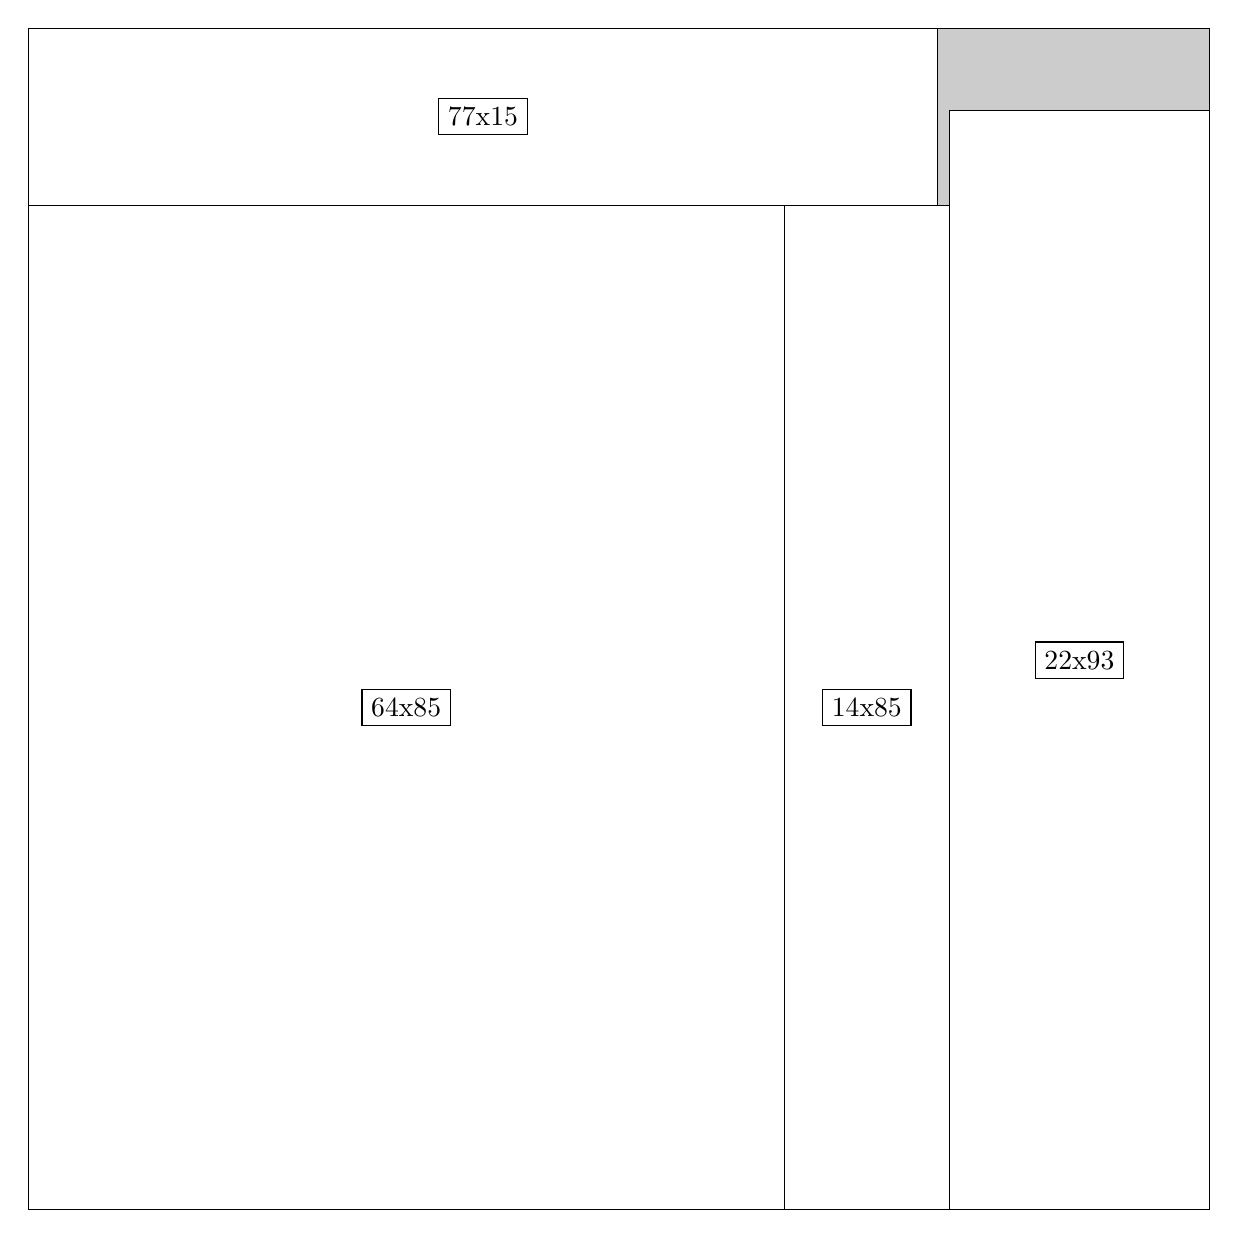
\begin{tikzpicture}[shorten >=1pt,scale=1.0,every node/.style={scale=1.0},->]
\tikzstyle{vertex}=[circle,fill=black!25,minimum size=14pt,inner sep=0pt]
\filldraw[fill=gray!40!white, draw=black] (0,0) rectangle (15.0,15.0);
\foreach \name/\x/\y/\w/\h in {64x85/0.0/0.0/9.6/12.75,22x93/11.7/0.0/3.3/13.95,14x85/9.6/0.0/2.1/12.75,77x15/0.0/12.75/11.549999999999999/2.25}
\filldraw[fill=white!40!white, draw=black] (\x,\y) rectangle node[draw] (\name) {\name} ++(\w,\h);
\end{tikzpicture}


w =64 , h =85 , x =0 , y =0 , v =5440
\par
w =22 , h =93 , x =78 , y =0 , v =2046
\par
w =14 , h =85 , x =64 , y =0 , v =1190
\par
w =77 , h =15 , x =0 , y =85 , v =1155
\par
\newpage


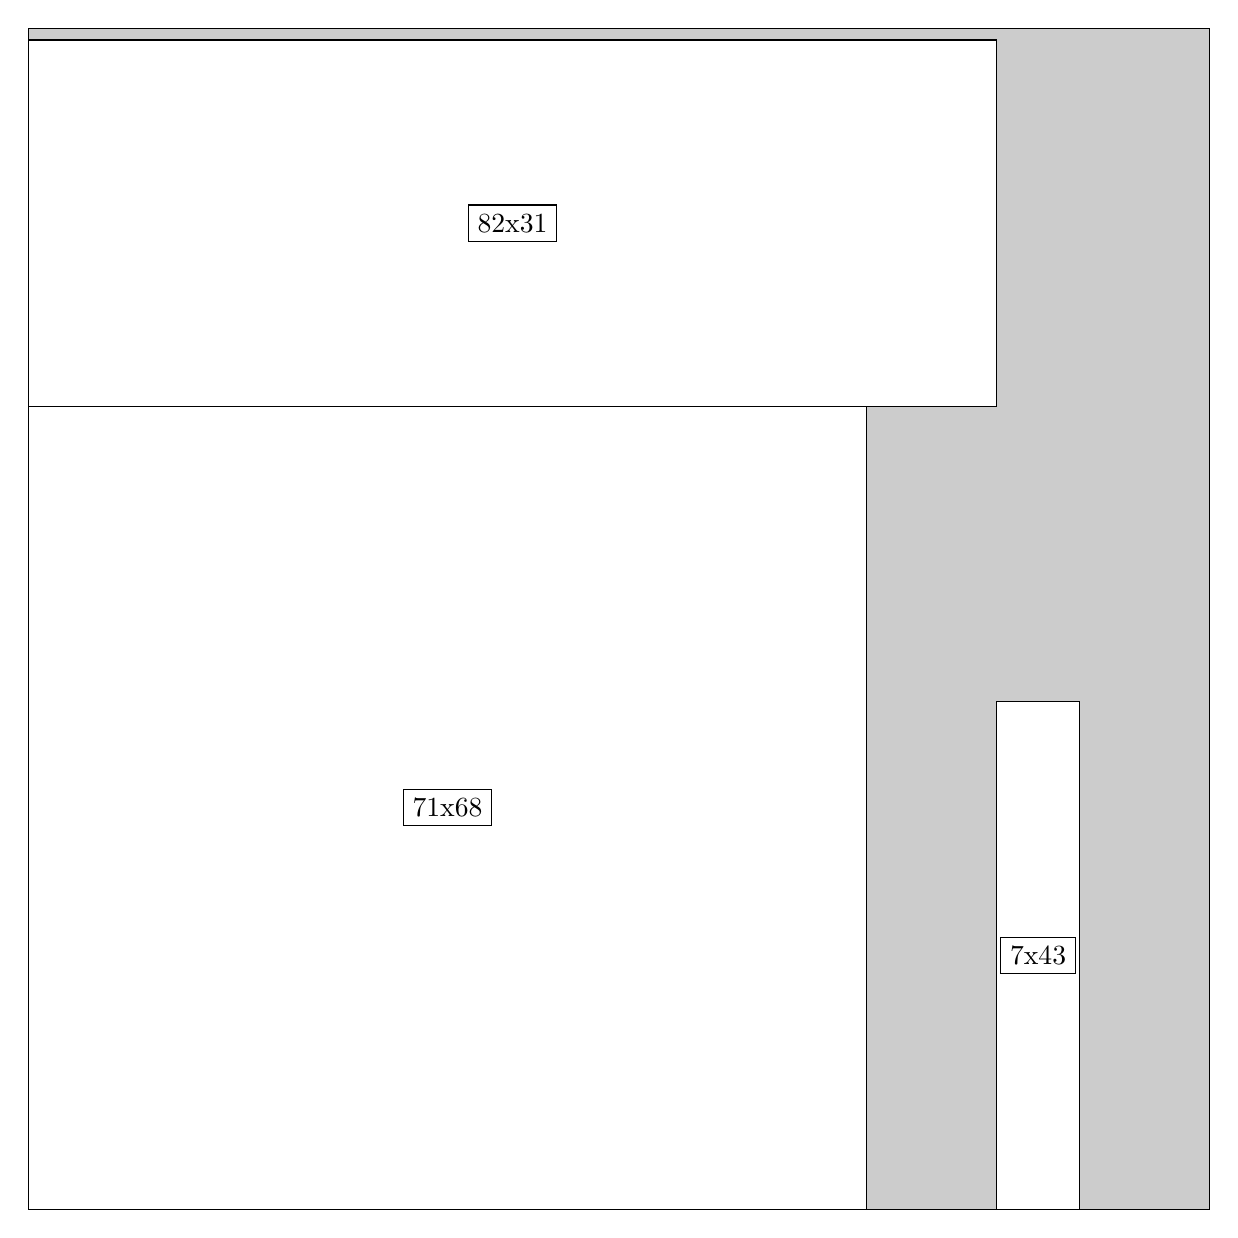
\begin{tikzpicture}[shorten >=1pt,scale=1.0,every node/.style={scale=1.0},->]
\tikzstyle{vertex}=[circle,fill=black!25,minimum size=14pt,inner sep=0pt]
\filldraw[fill=gray!40!white, draw=black] (0,0) rectangle (15.0,15.0);
\foreach \name/\x/\y/\w/\h in {71x68/0.0/0.0/10.65/10.2,82x31/0.0/10.2/12.299999999999999/4.6499999999999995,7x43/12.299999999999999/0.0/1.05/6.45}
\filldraw[fill=white!40!white, draw=black] (\x,\y) rectangle node[draw] (\name) {\name} ++(\w,\h);
\end{tikzpicture}


w =71 , h =68 , x =0 , y =0 , v =4828
\par
w =82 , h =31 , x =0 , y =68 , v =2542
\par
w =7 , h =43 , x =82 , y =0 , v =301
\par
\newpage


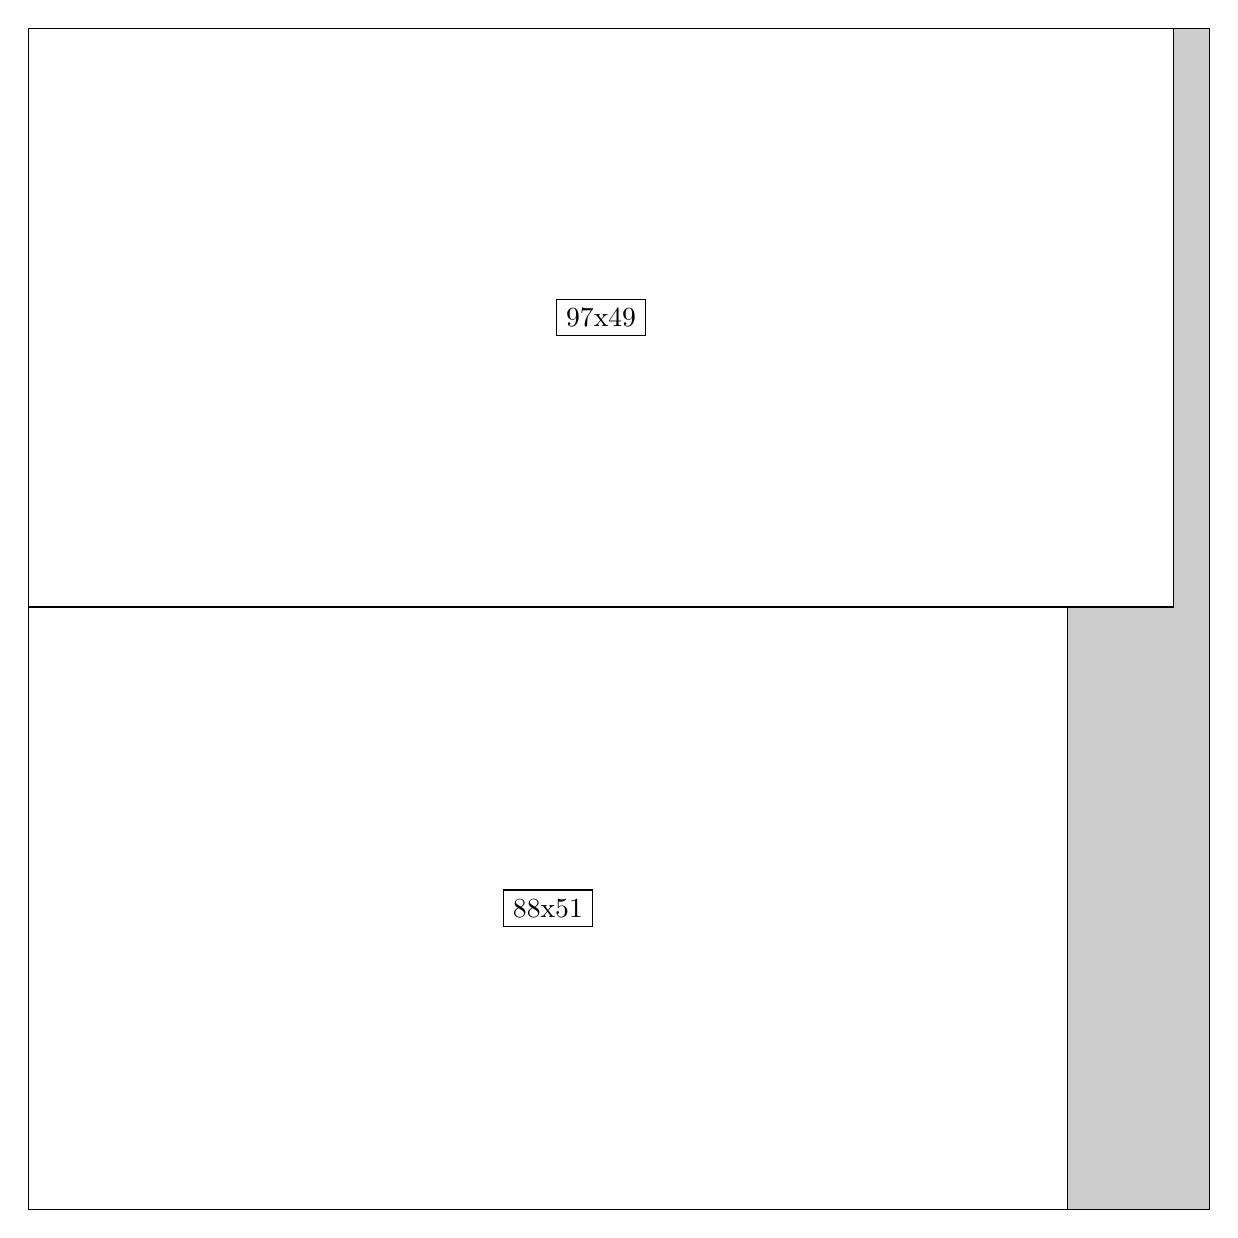
\begin{tikzpicture}[shorten >=1pt,scale=1.0,every node/.style={scale=1.0},->]
\tikzstyle{vertex}=[circle,fill=black!25,minimum size=14pt,inner sep=0pt]
\filldraw[fill=gray!40!white, draw=black] (0,0) rectangle (15.0,15.0);
\foreach \name/\x/\y/\w/\h in {97x49/0.0/7.6499999999999995/14.549999999999999/7.35,88x51/0.0/0.0/13.2/7.6499999999999995}
\filldraw[fill=white!40!white, draw=black] (\x,\y) rectangle node[draw] (\name) {\name} ++(\w,\h);
\end{tikzpicture}


w =97 , h =49 , x =0 , y =51 , v =4753
\par
w =88 , h =51 , x =0 , y =0 , v =4488
\par
\newpage


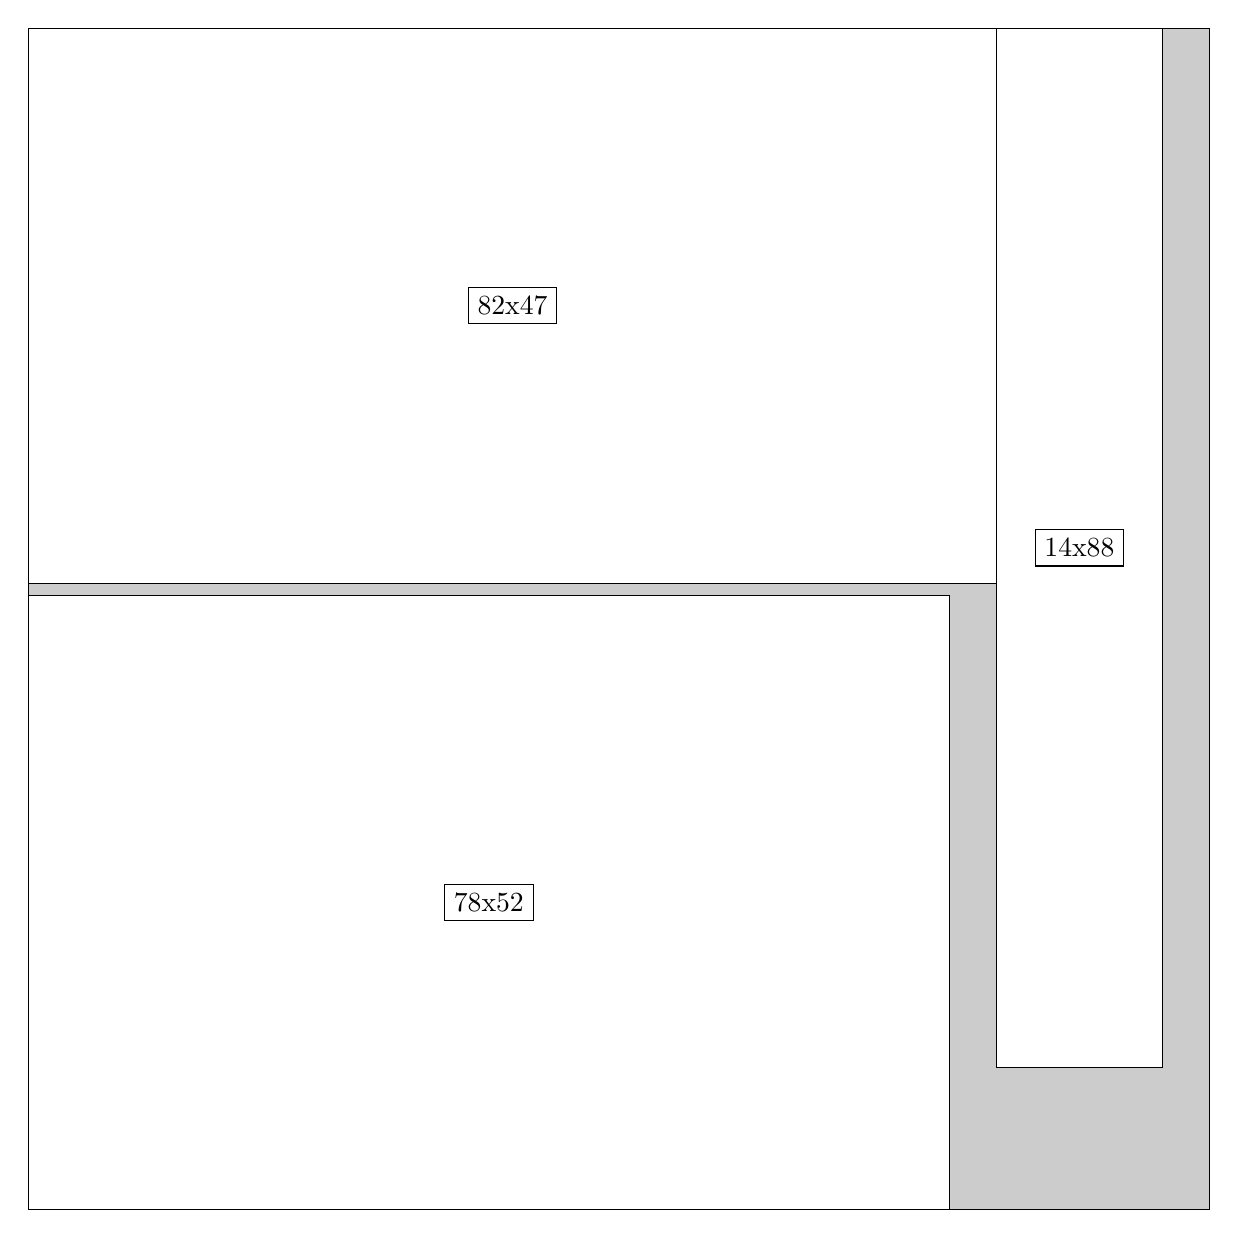
\begin{tikzpicture}[shorten >=1pt,scale=1.0,every node/.style={scale=1.0},->]
\tikzstyle{vertex}=[circle,fill=black!25,minimum size=14pt,inner sep=0pt]
\filldraw[fill=gray!40!white, draw=black] (0,0) rectangle (15.0,15.0);
\foreach \name/\x/\y/\w/\h in {78x52/0.0/0.0/11.7/7.8,82x47/0.0/7.949999999999999/12.299999999999999/7.05,14x88/12.299999999999999/1.7999999999999998/2.1/13.2}
\filldraw[fill=white!40!white, draw=black] (\x,\y) rectangle node[draw] (\name) {\name} ++(\w,\h);
\end{tikzpicture}


w =78 , h =52 , x =0 , y =0 , v =4056
\par
w =82 , h =47 , x =0 , y =53 , v =3854
\par
w =14 , h =88 , x =82 , y =12 , v =1232
\par
\newpage


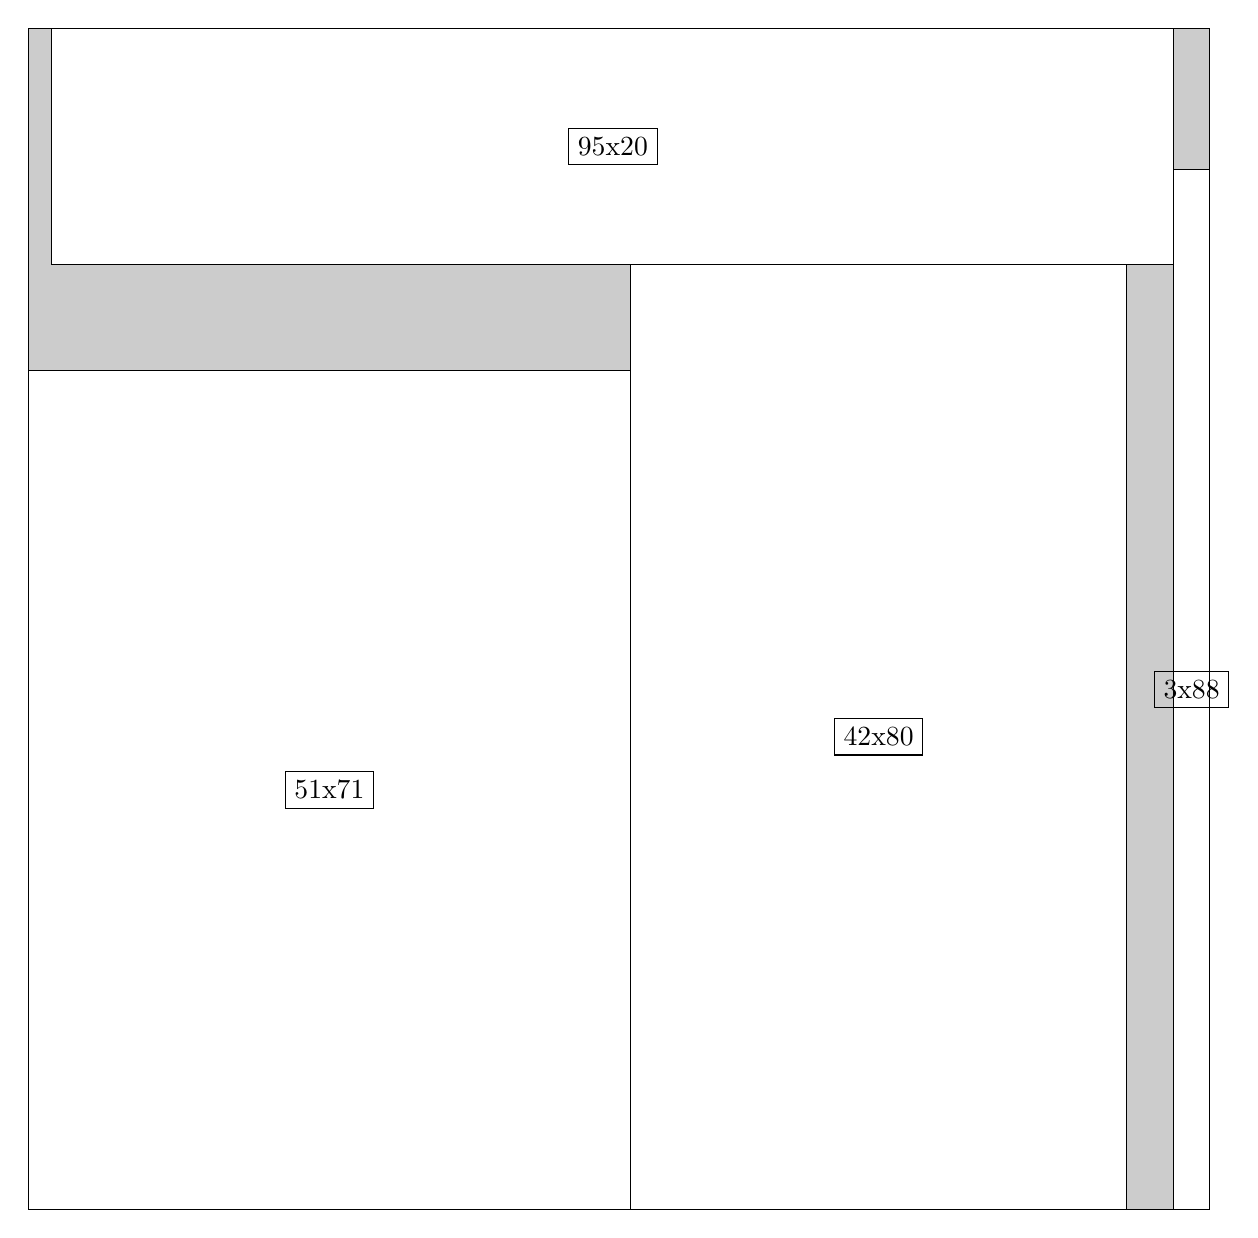
\begin{tikzpicture}[shorten >=1pt,scale=1.0,every node/.style={scale=1.0},->]
\tikzstyle{vertex}=[circle,fill=black!25,minimum size=14pt,inner sep=0pt]
\filldraw[fill=gray!40!white, draw=black] (0,0) rectangle (15.0,15.0);
\foreach \name/\x/\y/\w/\h in {51x71/0.0/0.0/7.6499999999999995/10.65,42x80/7.6499999999999995/0.0/6.3/12.0,95x20/0.3/12.0/14.25/3.0,3x88/14.549999999999999/0.0/0.44999999999999996/13.2}
\filldraw[fill=white!40!white, draw=black] (\x,\y) rectangle node[draw] (\name) {\name} ++(\w,\h);
\end{tikzpicture}


w =51 , h =71 , x =0 , y =0 , v =3621
\par
w =42 , h =80 , x =51 , y =0 , v =3360
\par
w =95 , h =20 , x =2 , y =80 , v =1900
\par
w =3 , h =88 , x =97 , y =0 , v =264
\par
\newpage


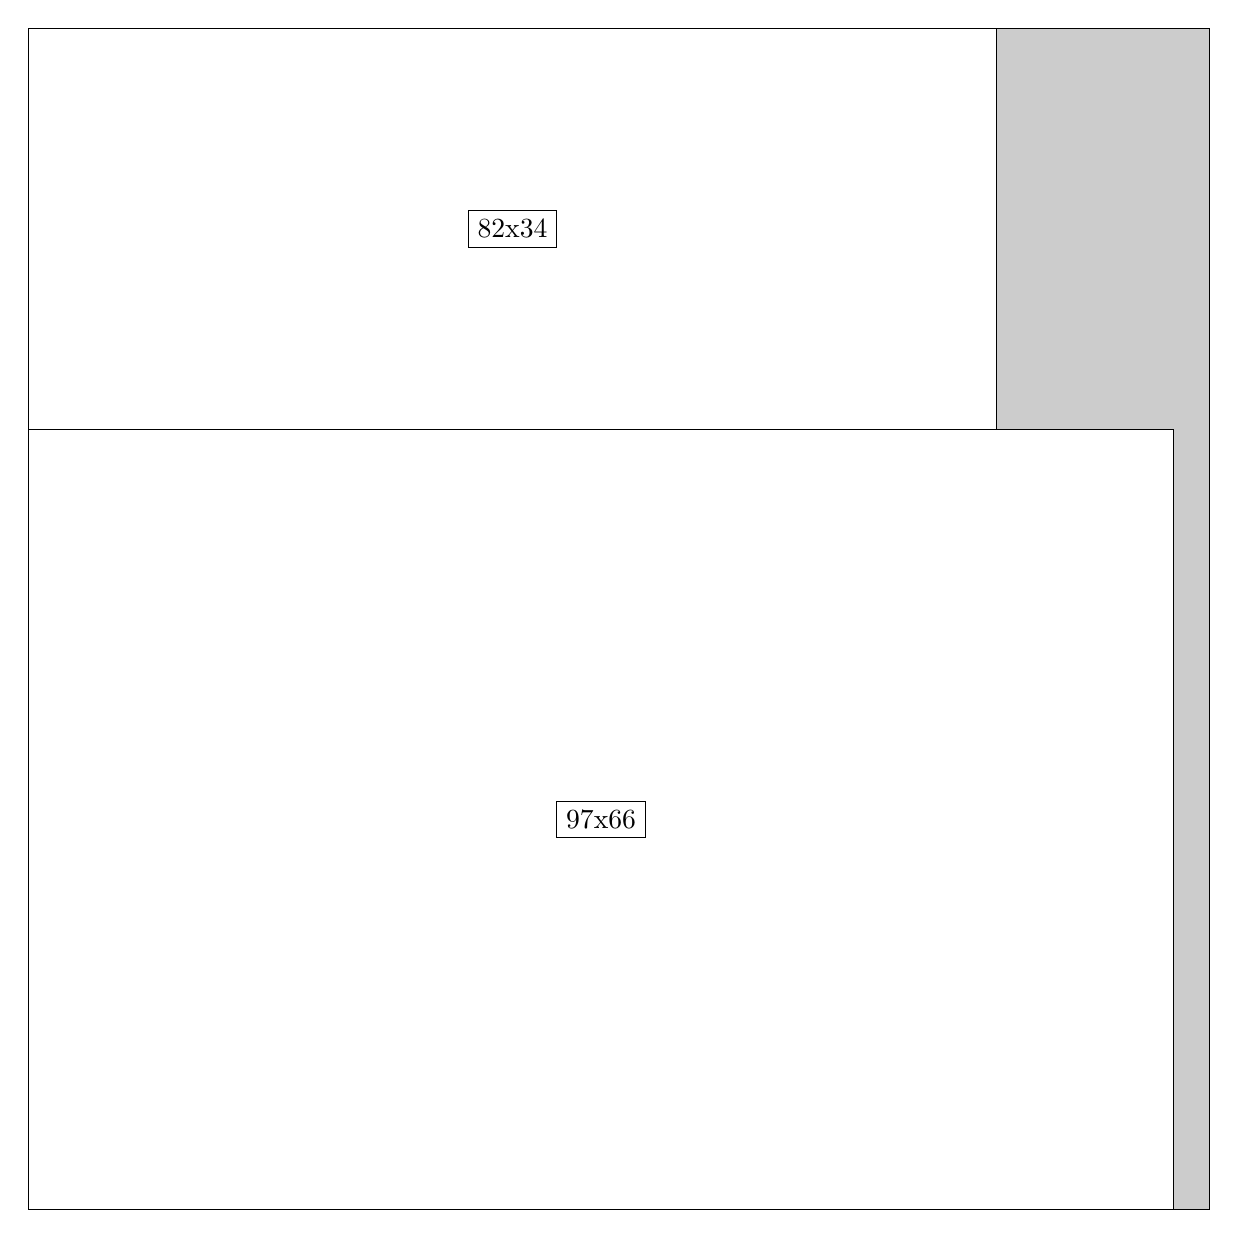
\begin{tikzpicture}[shorten >=1pt,scale=1.0,every node/.style={scale=1.0},->]
\tikzstyle{vertex}=[circle,fill=black!25,minimum size=14pt,inner sep=0pt]
\filldraw[fill=gray!40!white, draw=black] (0,0) rectangle (15.0,15.0);
\foreach \name/\x/\y/\w/\h in {97x66/0.0/0.0/14.549999999999999/9.9,82x34/0.0/9.9/12.299999999999999/5.1}
\filldraw[fill=white!40!white, draw=black] (\x,\y) rectangle node[draw] (\name) {\name} ++(\w,\h);
\end{tikzpicture}


w =97 , h =66 , x =0 , y =0 , v =6402
\par
w =82 , h =34 , x =0 , y =66 , v =2788
\par
\newpage


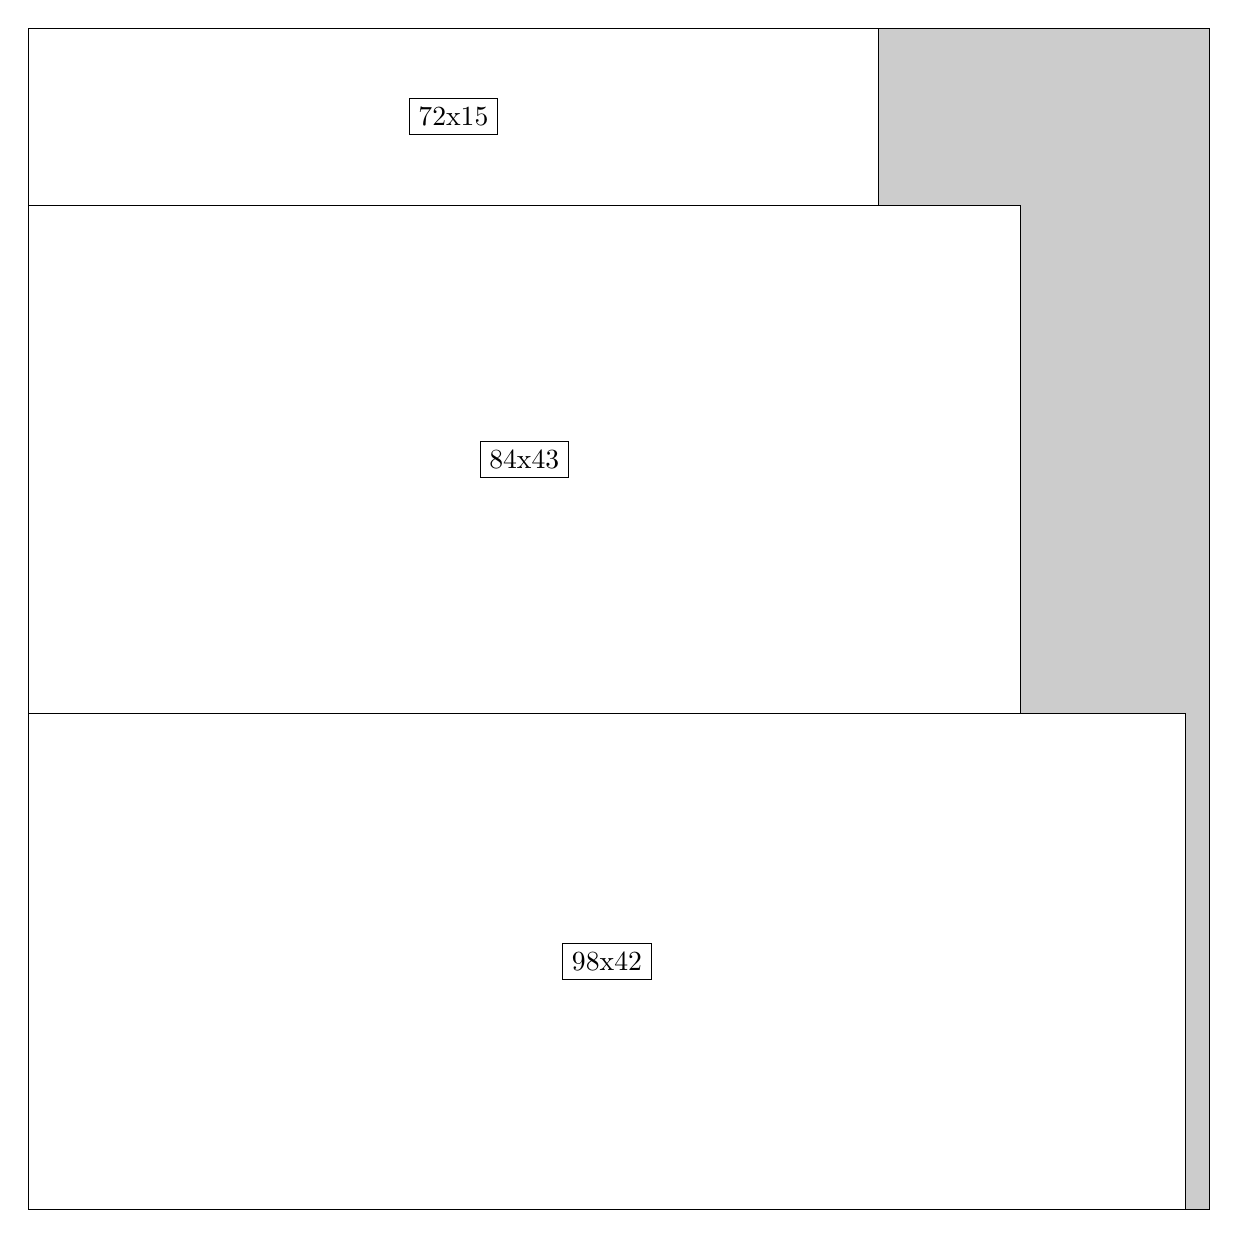
\begin{tikzpicture}[shorten >=1pt,scale=1.0,every node/.style={scale=1.0},->]
\tikzstyle{vertex}=[circle,fill=black!25,minimum size=14pt,inner sep=0pt]
\filldraw[fill=gray!40!white, draw=black] (0,0) rectangle (15.0,15.0);
\foreach \name/\x/\y/\w/\h in {98x42/0.0/0.0/14.7/6.3,84x43/0.0/6.3/12.6/6.45,72x15/0.0/12.75/10.799999999999999/2.25}
\filldraw[fill=white!40!white, draw=black] (\x,\y) rectangle node[draw] (\name) {\name} ++(\w,\h);
\end{tikzpicture}


w =98 , h =42 , x =0 , y =0 , v =4116
\par
w =84 , h =43 , x =0 , y =42 , v =3612
\par
w =72 , h =15 , x =0 , y =85 , v =1080
\par
\newpage


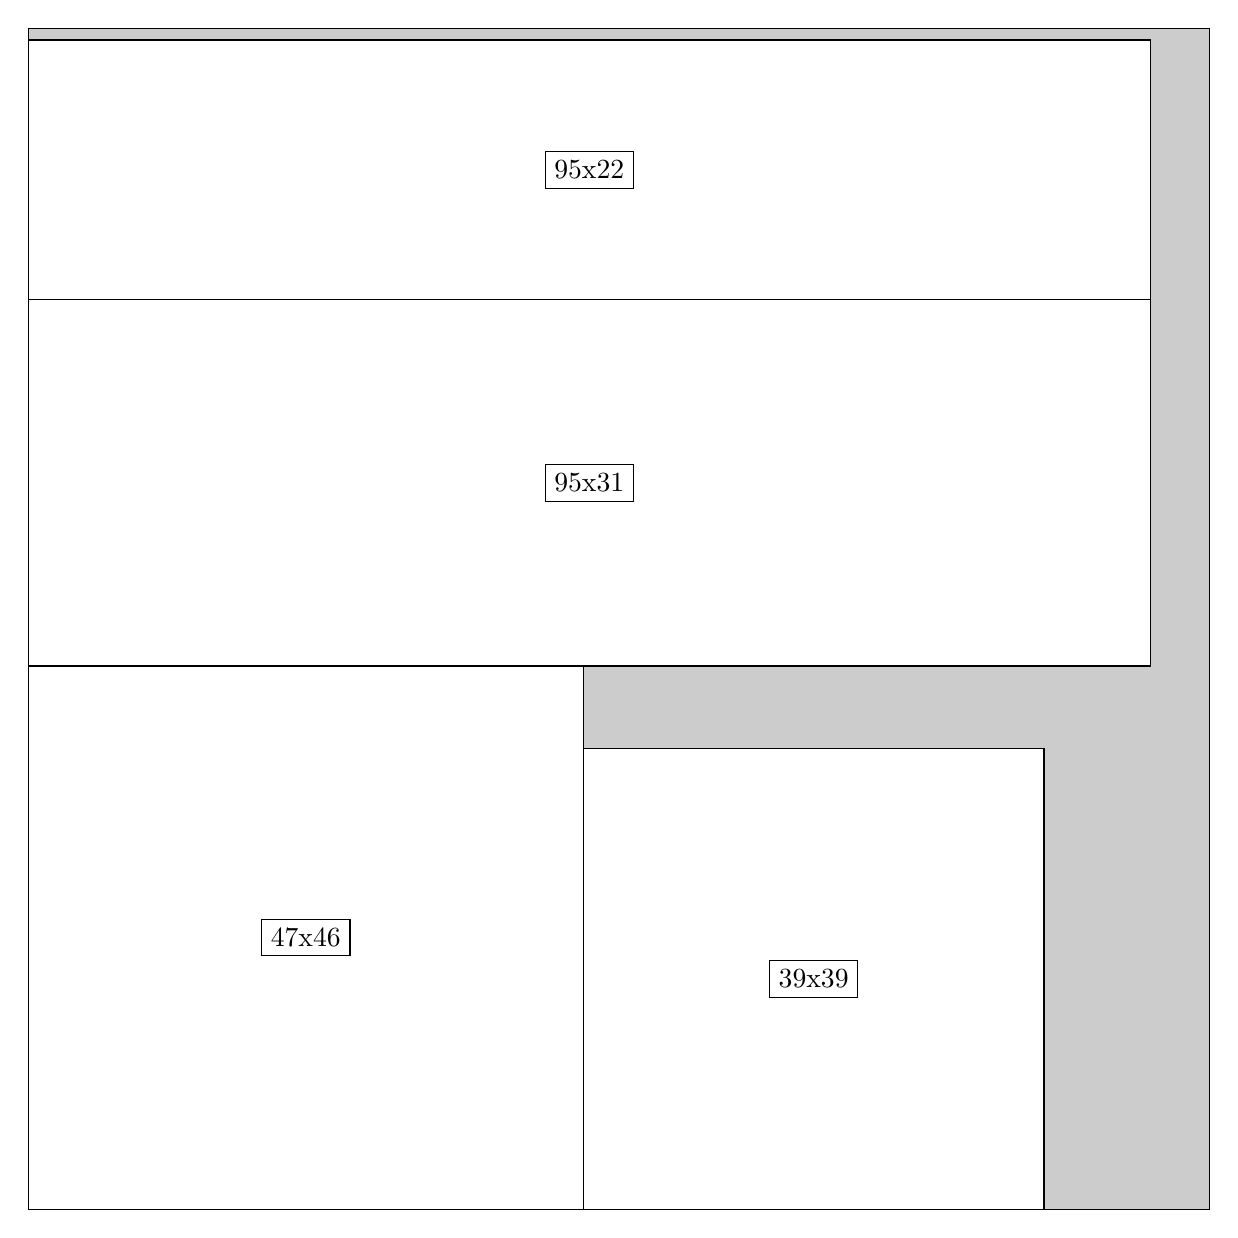
\begin{tikzpicture}[shorten >=1pt,scale=1.0,every node/.style={scale=1.0},->]
\tikzstyle{vertex}=[circle,fill=black!25,minimum size=14pt,inner sep=0pt]
\filldraw[fill=gray!40!white, draw=black] (0,0) rectangle (15.0,15.0);
\foreach \name/\x/\y/\w/\h in {95x31/0.0/6.8999999999999995/14.25/4.6499999999999995,47x46/0.0/0.0/7.05/6.8999999999999995,95x22/0.0/11.549999999999999/14.25/3.3,39x39/7.05/0.0/5.85/5.85}
\filldraw[fill=white!40!white, draw=black] (\x,\y) rectangle node[draw] (\name) {\name} ++(\w,\h);
\end{tikzpicture}


w =95 , h =31 , x =0 , y =46 , v =2945
\par
w =47 , h =46 , x =0 , y =0 , v =2162
\par
w =95 , h =22 , x =0 , y =77 , v =2090
\par
w =39 , h =39 , x =47 , y =0 , v =1521
\par
\newpage


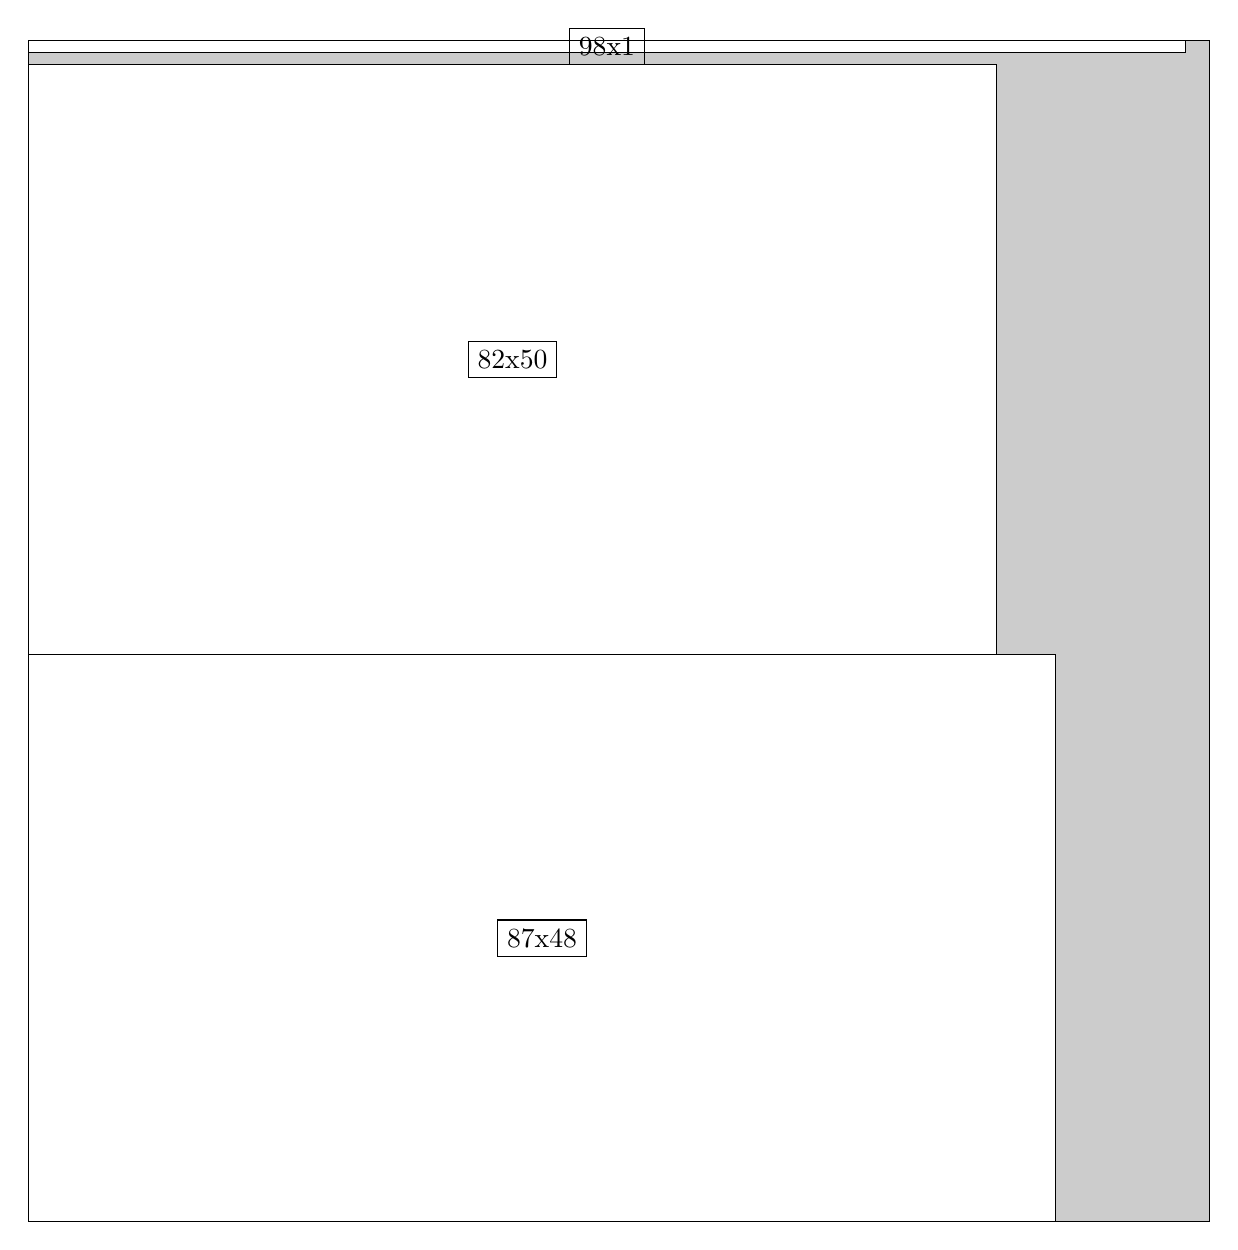
\begin{tikzpicture}[shorten >=1pt,scale=1.0,every node/.style={scale=1.0},->]
\tikzstyle{vertex}=[circle,fill=black!25,minimum size=14pt,inner sep=0pt]
\filldraw[fill=gray!40!white, draw=black] (0,0) rectangle (15.0,15.0);
\foreach \name/\x/\y/\w/\h in {87x48/0.0/0.0/13.049999999999999/7.199999999999999,82x50/0.0/7.199999999999999/12.299999999999999/7.5,98x1/0.0/14.85/14.7/0.15}
\filldraw[fill=white!40!white, draw=black] (\x,\y) rectangle node[draw] (\name) {\name} ++(\w,\h);
\end{tikzpicture}


w =87 , h =48 , x =0 , y =0 , v =4176
\par
w =82 , h =50 , x =0 , y =48 , v =4100
\par
w =98 , h =1 , x =0 , y =99 , v =98
\par
\newpage


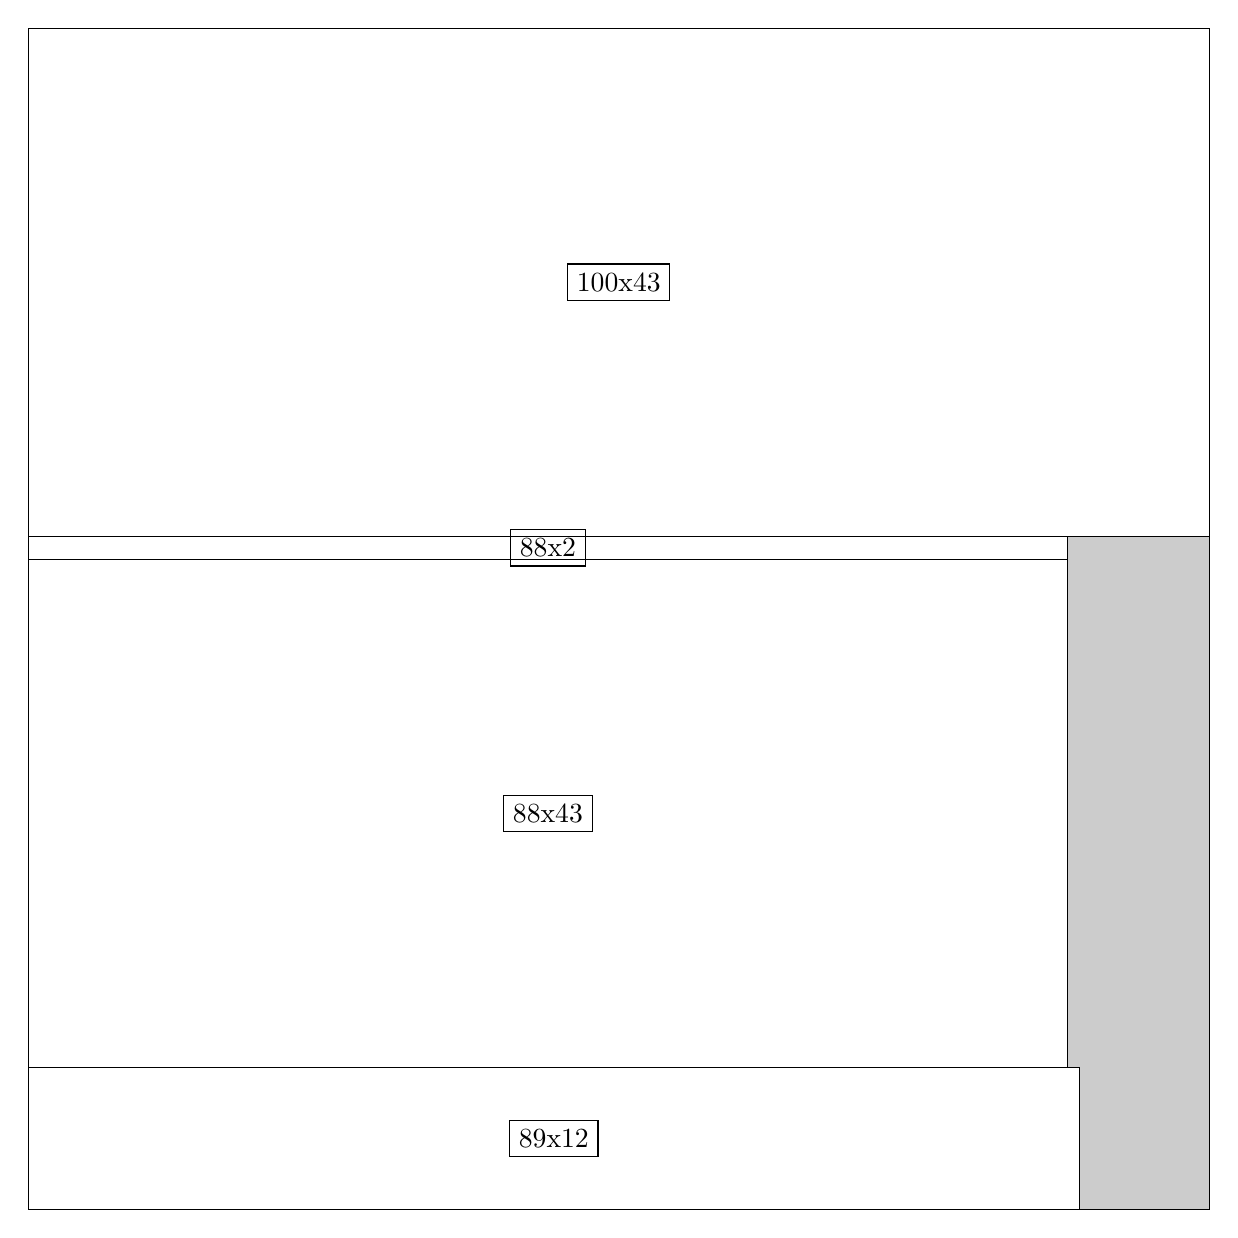
\begin{tikzpicture}[shorten >=1pt,scale=1.0,every node/.style={scale=1.0},->]
\tikzstyle{vertex}=[circle,fill=black!25,minimum size=14pt,inner sep=0pt]
\filldraw[fill=gray!40!white, draw=black] (0,0) rectangle (15.0,15.0);
\foreach \name/\x/\y/\w/\h in {100x43/0.0/8.549999999999999/15.0/6.45,88x43/0.0/1.7999999999999998/13.2/6.45,89x12/0.0/0.0/13.35/1.7999999999999998,88x2/0.0/8.25/13.2/0.3}
\filldraw[fill=white!40!white, draw=black] (\x,\y) rectangle node[draw] (\name) {\name} ++(\w,\h);
\end{tikzpicture}


w =100 , h =43 , x =0 , y =57 , v =4300
\par
w =88 , h =43 , x =0 , y =12 , v =3784
\par
w =89 , h =12 , x =0 , y =0 , v =1068
\par
w =88 , h =2 , x =0 , y =55 , v =176
\par
\newpage


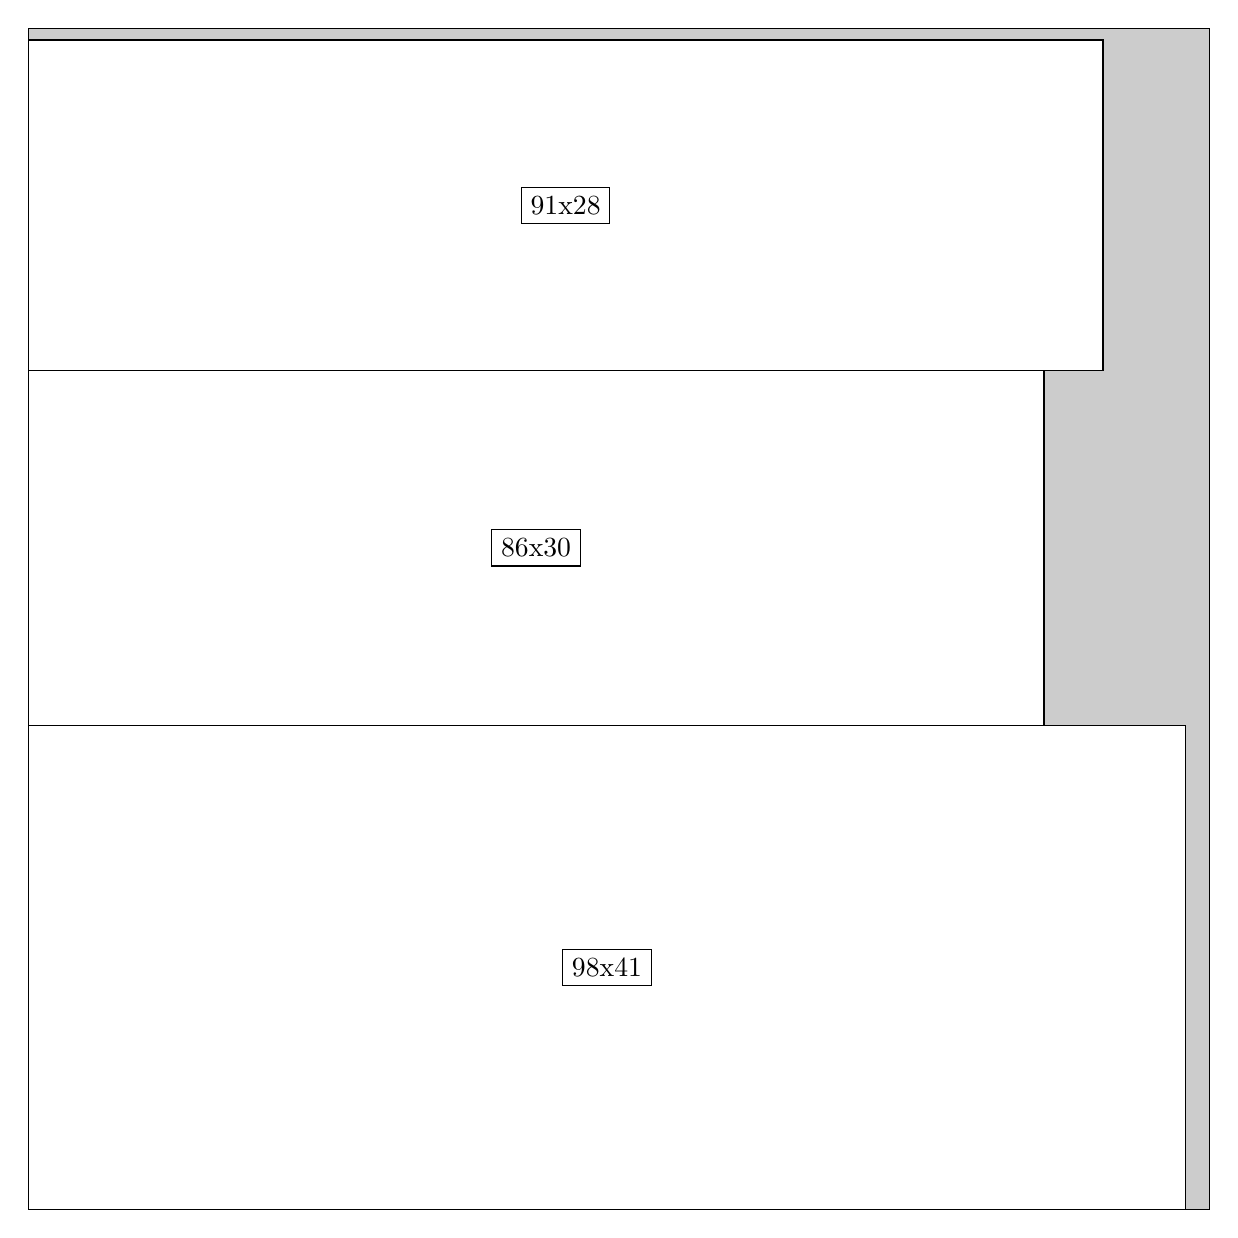
\begin{tikzpicture}[shorten >=1pt,scale=1.0,every node/.style={scale=1.0},->]
\tikzstyle{vertex}=[circle,fill=black!25,minimum size=14pt,inner sep=0pt]
\filldraw[fill=gray!40!white, draw=black] (0,0) rectangle (15.0,15.0);
\foreach \name/\x/\y/\w/\h in {98x41/0.0/0.0/14.7/6.1499999999999995,86x30/0.0/6.1499999999999995/12.9/4.5,91x28/0.0/10.65/13.65/4.2}
\filldraw[fill=white!40!white, draw=black] (\x,\y) rectangle node[draw] (\name) {\name} ++(\w,\h);
\end{tikzpicture}


w =98 , h =41 , x =0 , y =0 , v =4018
\par
w =86 , h =30 , x =0 , y =41 , v =2580
\par
w =91 , h =28 , x =0 , y =71 , v =2548
\par
\newpage


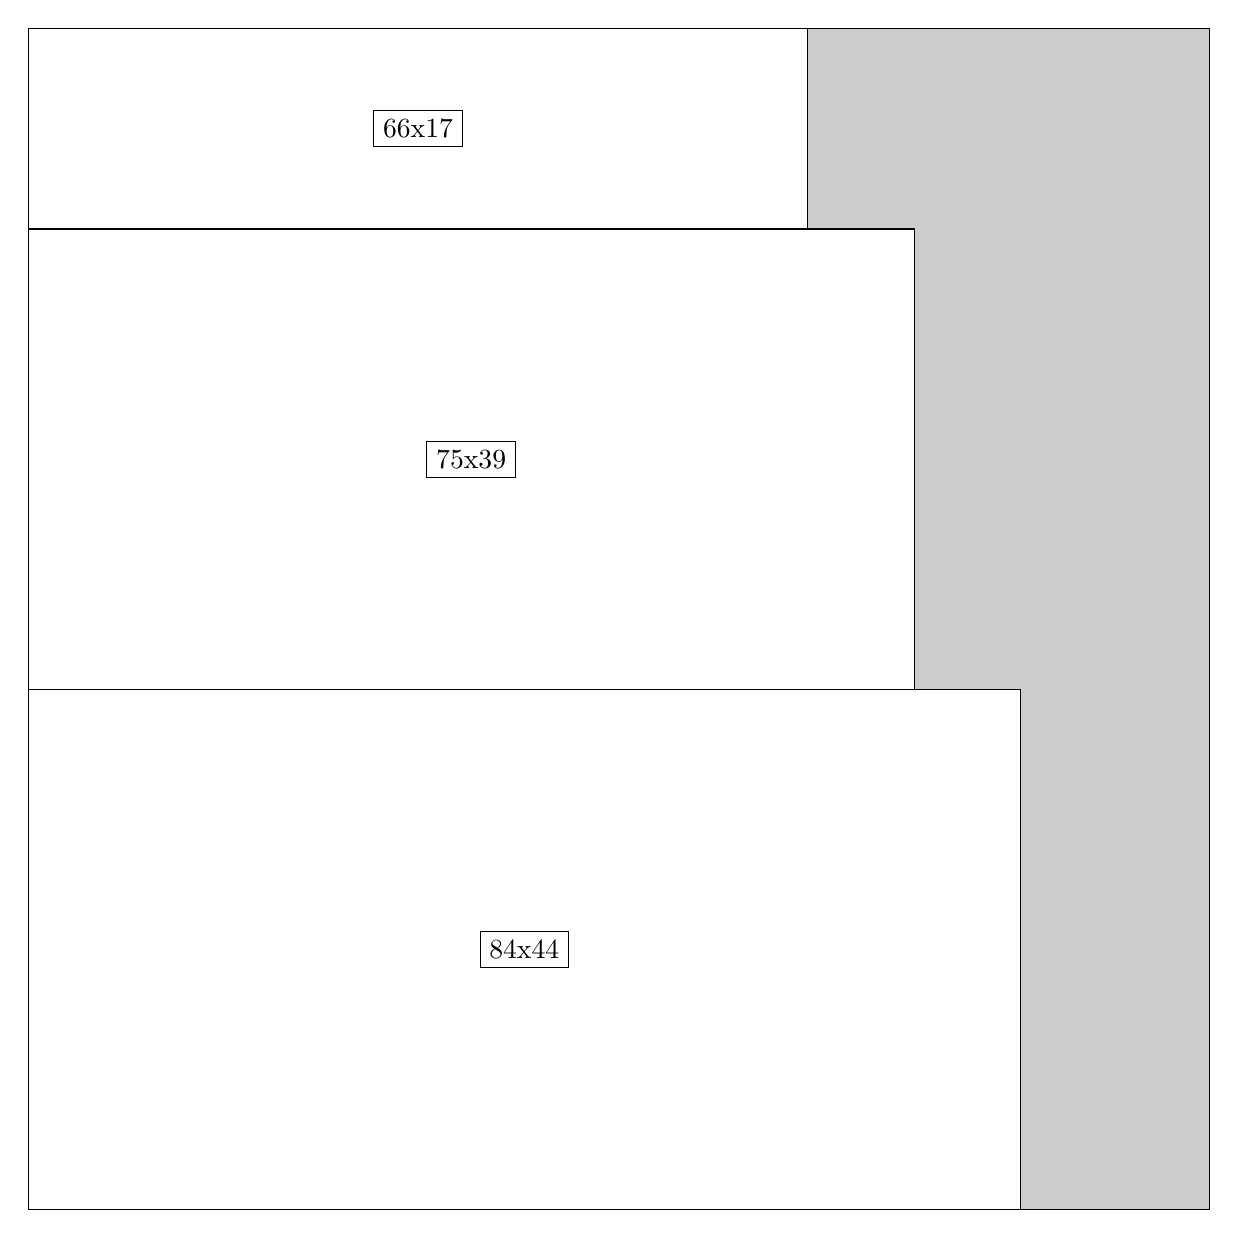
\begin{tikzpicture}[shorten >=1pt,scale=1.0,every node/.style={scale=1.0},->]
\tikzstyle{vertex}=[circle,fill=black!25,minimum size=14pt,inner sep=0pt]
\filldraw[fill=gray!40!white, draw=black] (0,0) rectangle (15.0,15.0);
\foreach \name/\x/\y/\w/\h in {84x44/0.0/0.0/12.6/6.6,75x39/0.0/6.6/11.25/5.85,66x17/0.0/12.45/9.9/2.55}
\filldraw[fill=white!40!white, draw=black] (\x,\y) rectangle node[draw] (\name) {\name} ++(\w,\h);
\end{tikzpicture}


w =84 , h =44 , x =0 , y =0 , v =3696
\par
w =75 , h =39 , x =0 , y =44 , v =2925
\par
w =66 , h =17 , x =0 , y =83 , v =1122
\par
\newpage


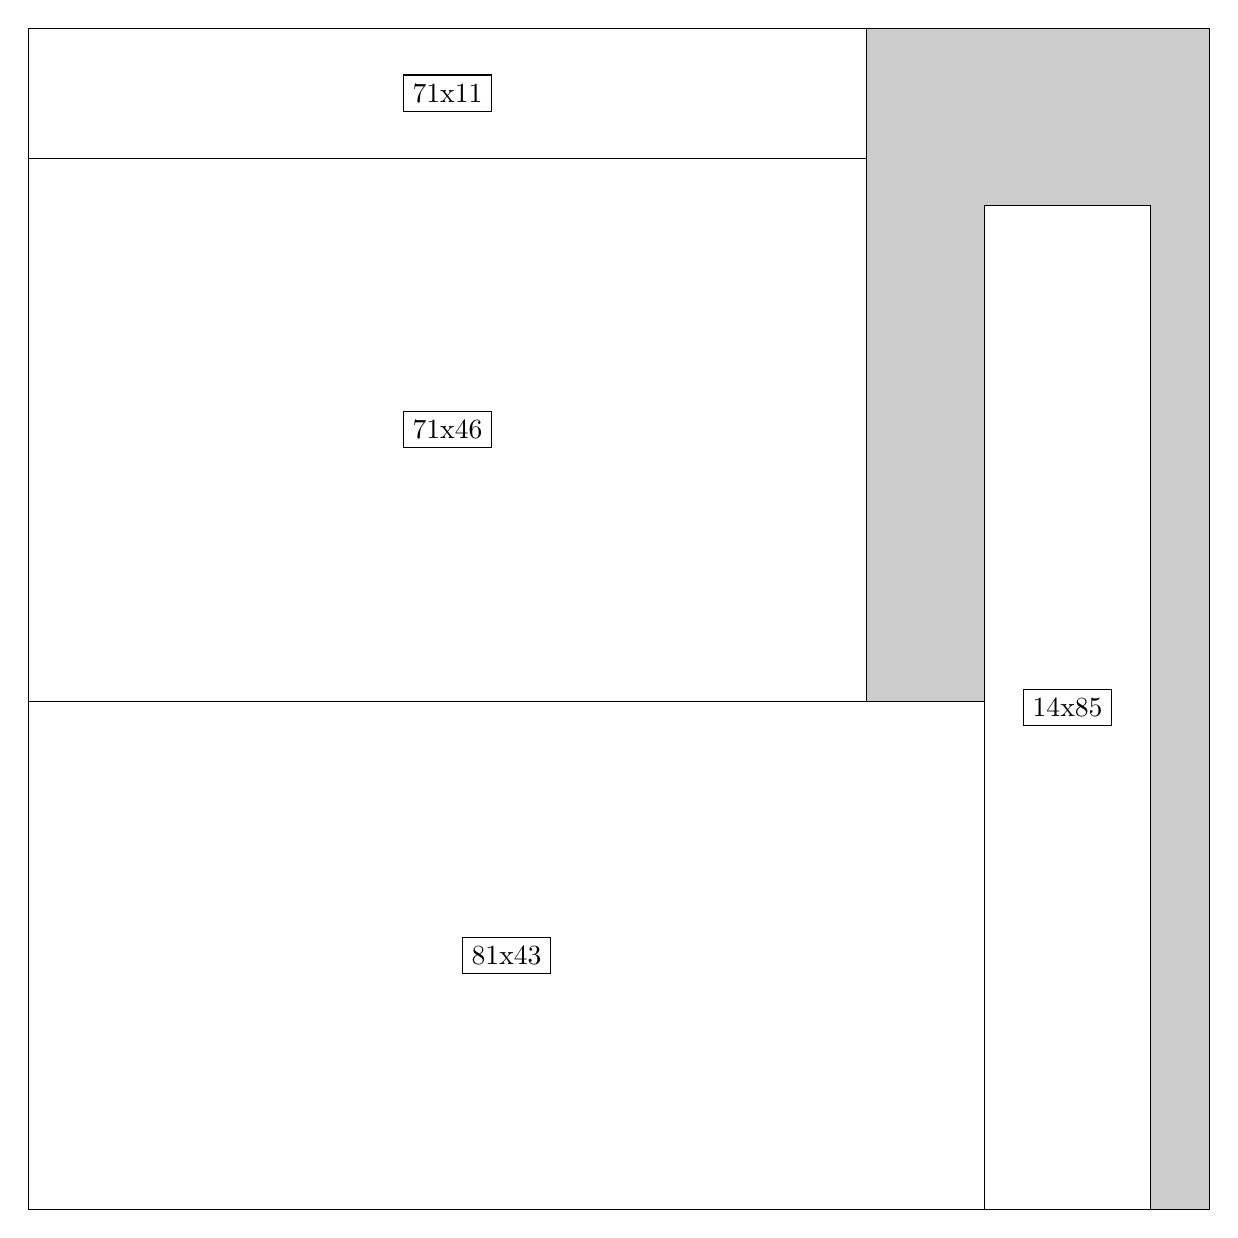
\begin{tikzpicture}[shorten >=1pt,scale=1.0,every node/.style={scale=1.0},->]
\tikzstyle{vertex}=[circle,fill=black!25,minimum size=14pt,inner sep=0pt]
\filldraw[fill=gray!40!white, draw=black] (0,0) rectangle (15.0,15.0);
\foreach \name/\x/\y/\w/\h in {81x43/0.0/0.0/12.15/6.45,71x46/0.0/6.45/10.65/6.8999999999999995,14x85/12.15/0.0/2.1/12.75,71x11/0.0/13.35/10.65/1.65}
\filldraw[fill=white!40!white, draw=black] (\x,\y) rectangle node[draw] (\name) {\name} ++(\w,\h);
\end{tikzpicture}


w =81 , h =43 , x =0 , y =0 , v =3483
\par
w =71 , h =46 , x =0 , y =43 , v =3266
\par
w =14 , h =85 , x =81 , y =0 , v =1190
\par
w =71 , h =11 , x =0 , y =89 , v =781
\par
\newpage


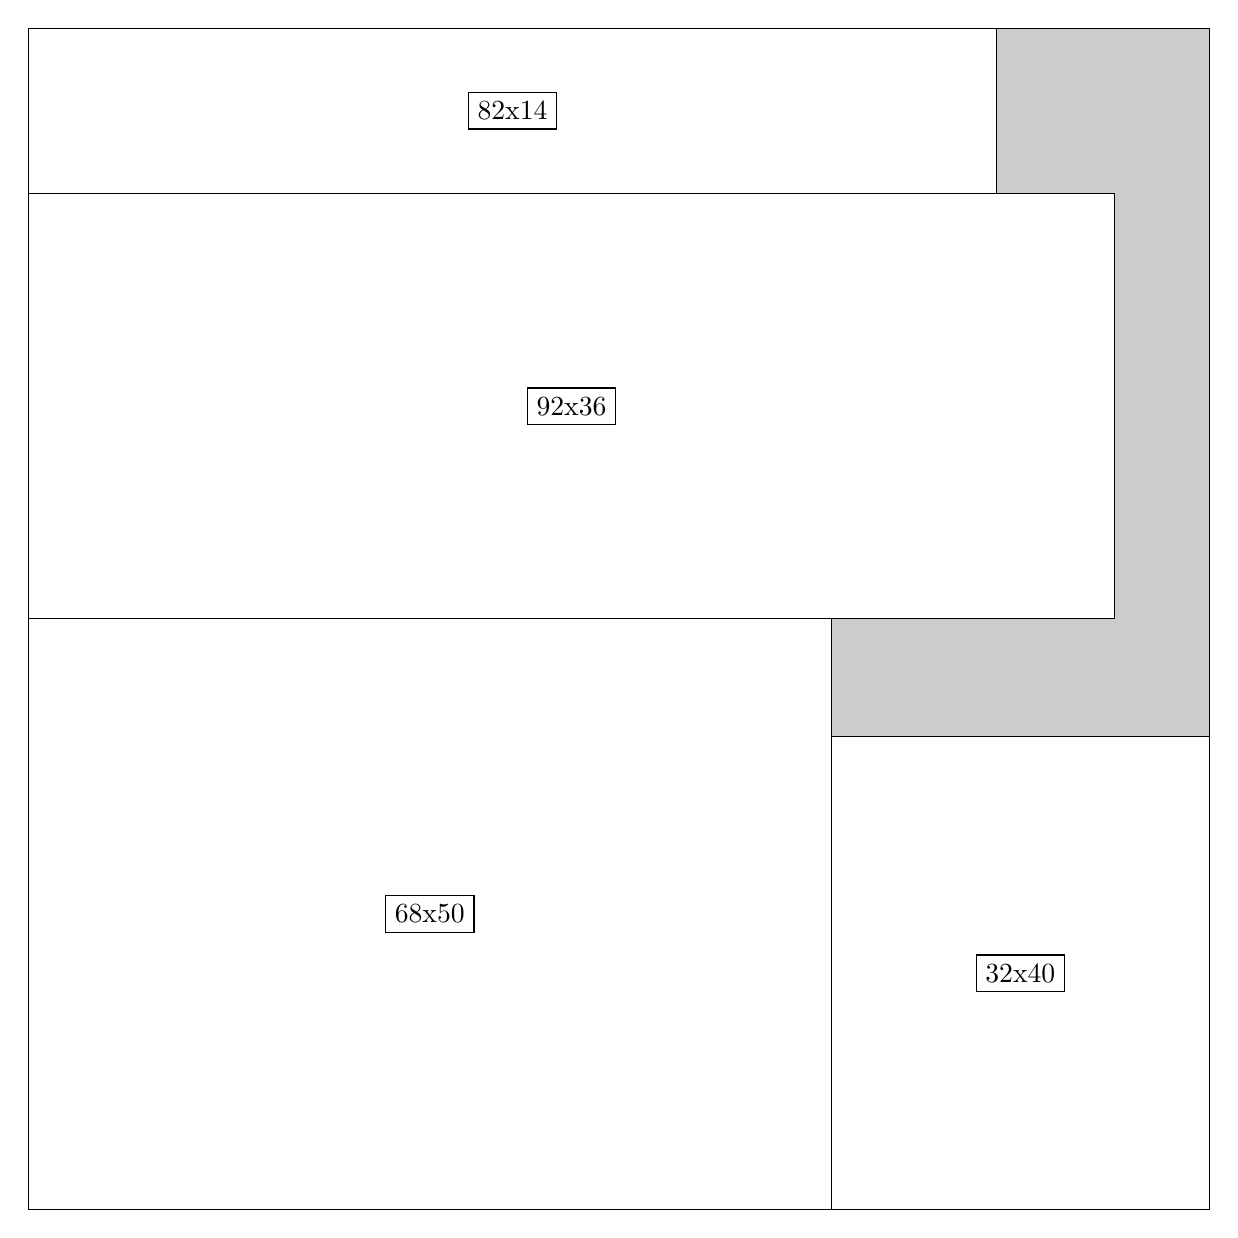
\begin{tikzpicture}[shorten >=1pt,scale=1.0,every node/.style={scale=1.0},->]
\tikzstyle{vertex}=[circle,fill=black!25,minimum size=14pt,inner sep=0pt]
\filldraw[fill=gray!40!white, draw=black] (0,0) rectangle (15.0,15.0);
\foreach \name/\x/\y/\w/\h in {68x50/0.0/0.0/10.2/7.5,92x36/0.0/7.5/13.799999999999999/5.3999999999999995,32x40/10.2/0.0/4.8/6.0,82x14/0.0/12.9/12.299999999999999/2.1}
\filldraw[fill=white!40!white, draw=black] (\x,\y) rectangle node[draw] (\name) {\name} ++(\w,\h);
\end{tikzpicture}


w =68 , h =50 , x =0 , y =0 , v =3400
\par
w =92 , h =36 , x =0 , y =50 , v =3312
\par
w =32 , h =40 , x =68 , y =0 , v =1280
\par
w =82 , h =14 , x =0 , y =86 , v =1148
\par
\newpage


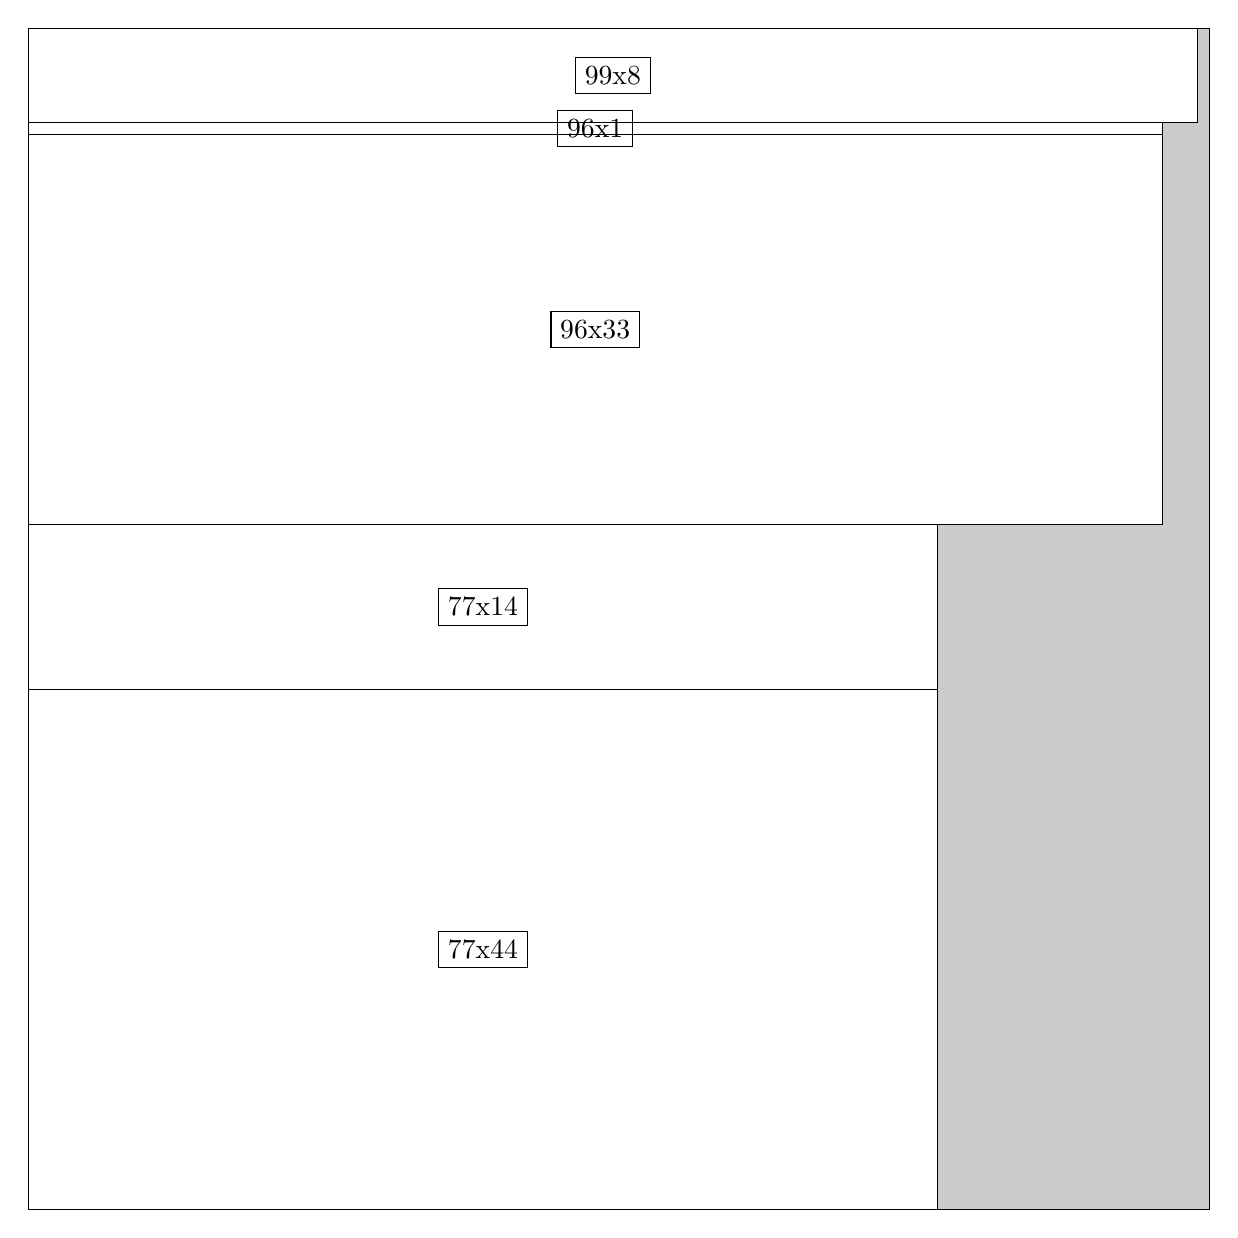
\begin{tikzpicture}[shorten >=1pt,scale=1.0,every node/.style={scale=1.0},->]
\tikzstyle{vertex}=[circle,fill=black!25,minimum size=14pt,inner sep=0pt]
\filldraw[fill=gray!40!white, draw=black] (0,0) rectangle (15.0,15.0);
\foreach \name/\x/\y/\w/\h in {77x44/0.0/0.0/11.549999999999999/6.6,96x33/0.0/8.7/14.399999999999999/4.95,77x14/0.0/6.6/11.549999999999999/2.1,99x8/0.0/13.799999999999999/14.85/1.2,96x1/0.0/13.65/14.399999999999999/0.15}
\filldraw[fill=white!40!white, draw=black] (\x,\y) rectangle node[draw] (\name) {\name} ++(\w,\h);
\end{tikzpicture}


w =77 , h =44 , x =0 , y =0 , v =3388
\par
w =96 , h =33 , x =0 , y =58 , v =3168
\par
w =77 , h =14 , x =0 , y =44 , v =1078
\par
w =99 , h =8 , x =0 , y =92 , v =792
\par
w =96 , h =1 , x =0 , y =91 , v =96
\par
\newpage


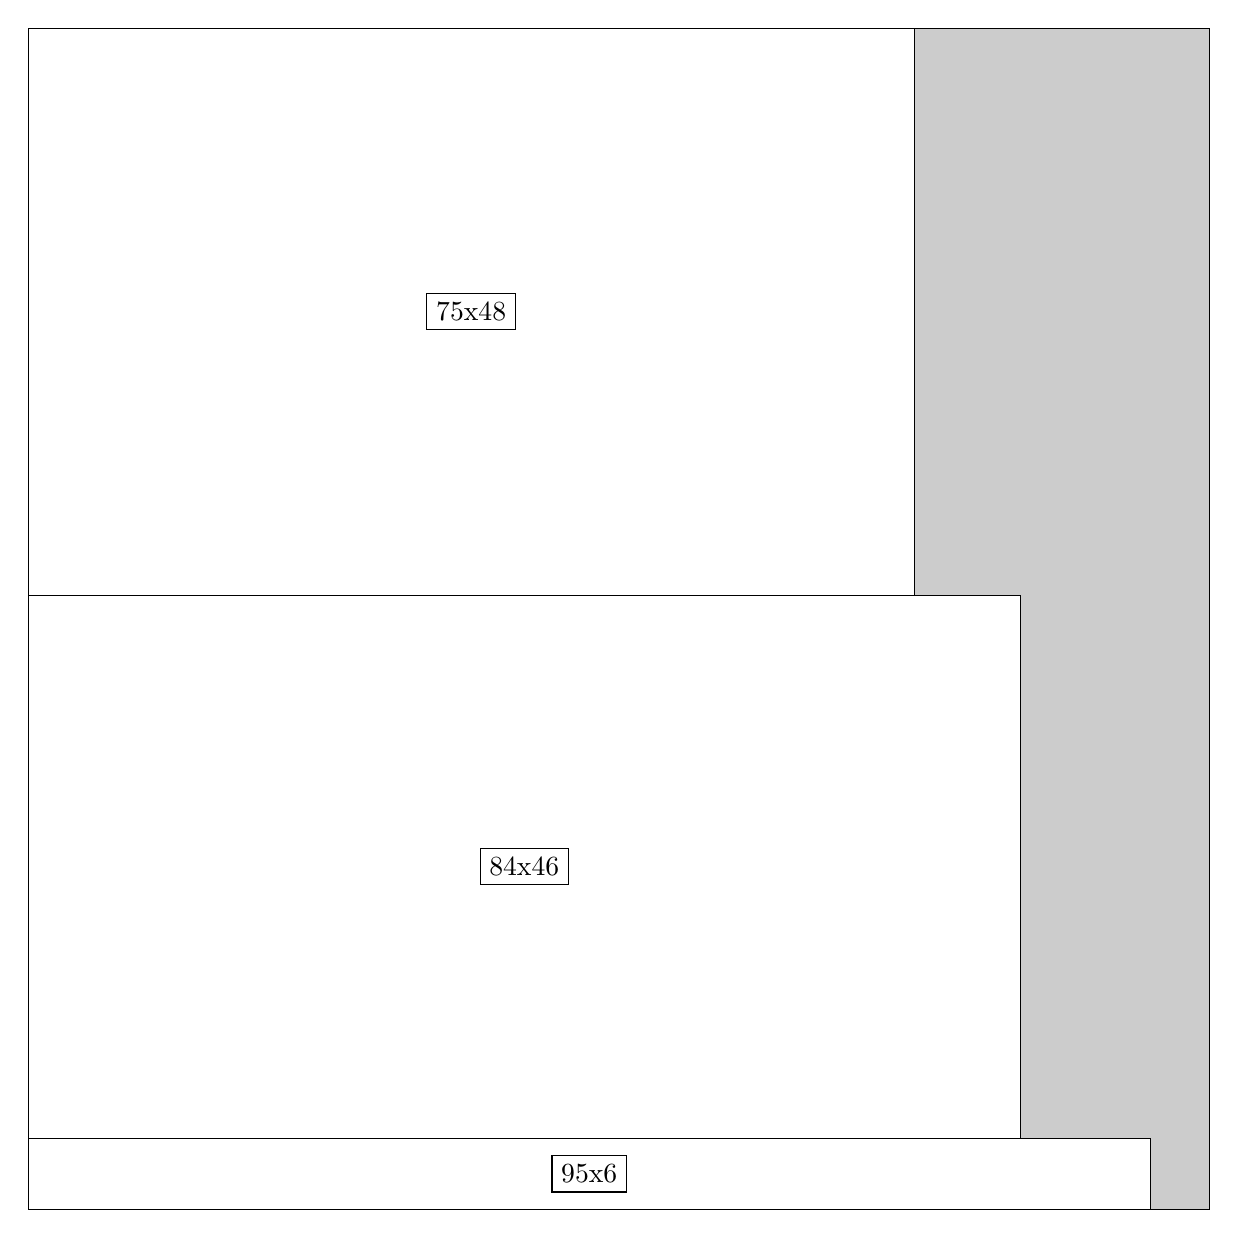
\begin{tikzpicture}[shorten >=1pt,scale=1.0,every node/.style={scale=1.0},->]
\tikzstyle{vertex}=[circle,fill=black!25,minimum size=14pt,inner sep=0pt]
\filldraw[fill=gray!40!white, draw=black] (0,0) rectangle (15.0,15.0);
\foreach \name/\x/\y/\w/\h in {84x46/0.0/0.8999999999999999/12.6/6.8999999999999995,75x48/0.0/7.8/11.25/7.199999999999999,95x6/0.0/0.0/14.25/0.8999999999999999}
\filldraw[fill=white!40!white, draw=black] (\x,\y) rectangle node[draw] (\name) {\name} ++(\w,\h);
\end{tikzpicture}


w =84 , h =46 , x =0 , y =6 , v =3864
\par
w =75 , h =48 , x =0 , y =52 , v =3600
\par
w =95 , h =6 , x =0 , y =0 , v =570
\par
\newpage


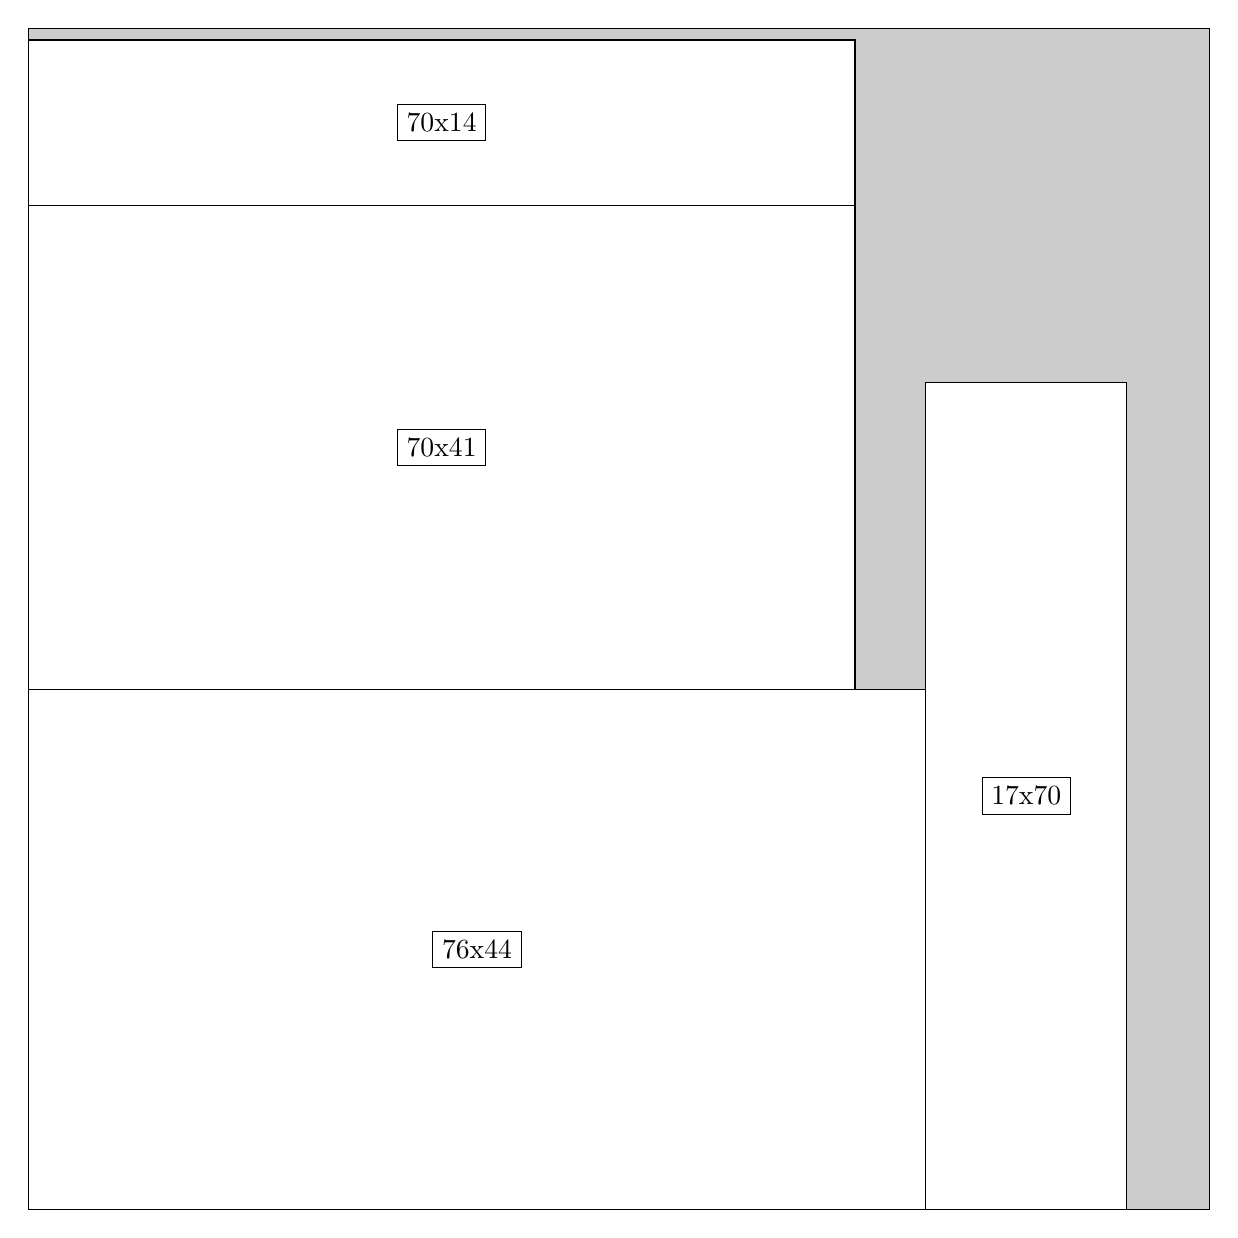
\begin{tikzpicture}[shorten >=1pt,scale=1.0,every node/.style={scale=1.0},->]
\tikzstyle{vertex}=[circle,fill=black!25,minimum size=14pt,inner sep=0pt]
\filldraw[fill=gray!40!white, draw=black] (0,0) rectangle (15.0,15.0);
\foreach \name/\x/\y/\w/\h in {76x44/0.0/0.0/11.4/6.6,70x41/0.0/6.6/10.5/6.1499999999999995,17x70/11.4/0.0/2.55/10.5,70x14/0.0/12.75/10.5/2.1}
\filldraw[fill=white!40!white, draw=black] (\x,\y) rectangle node[draw] (\name) {\name} ++(\w,\h);
\end{tikzpicture}


w =76 , h =44 , x =0 , y =0 , v =3344
\par
w =70 , h =41 , x =0 , y =44 , v =2870
\par
w =17 , h =70 , x =76 , y =0 , v =1190
\par
w =70 , h =14 , x =0 , y =85 , v =980
\par
\newpage


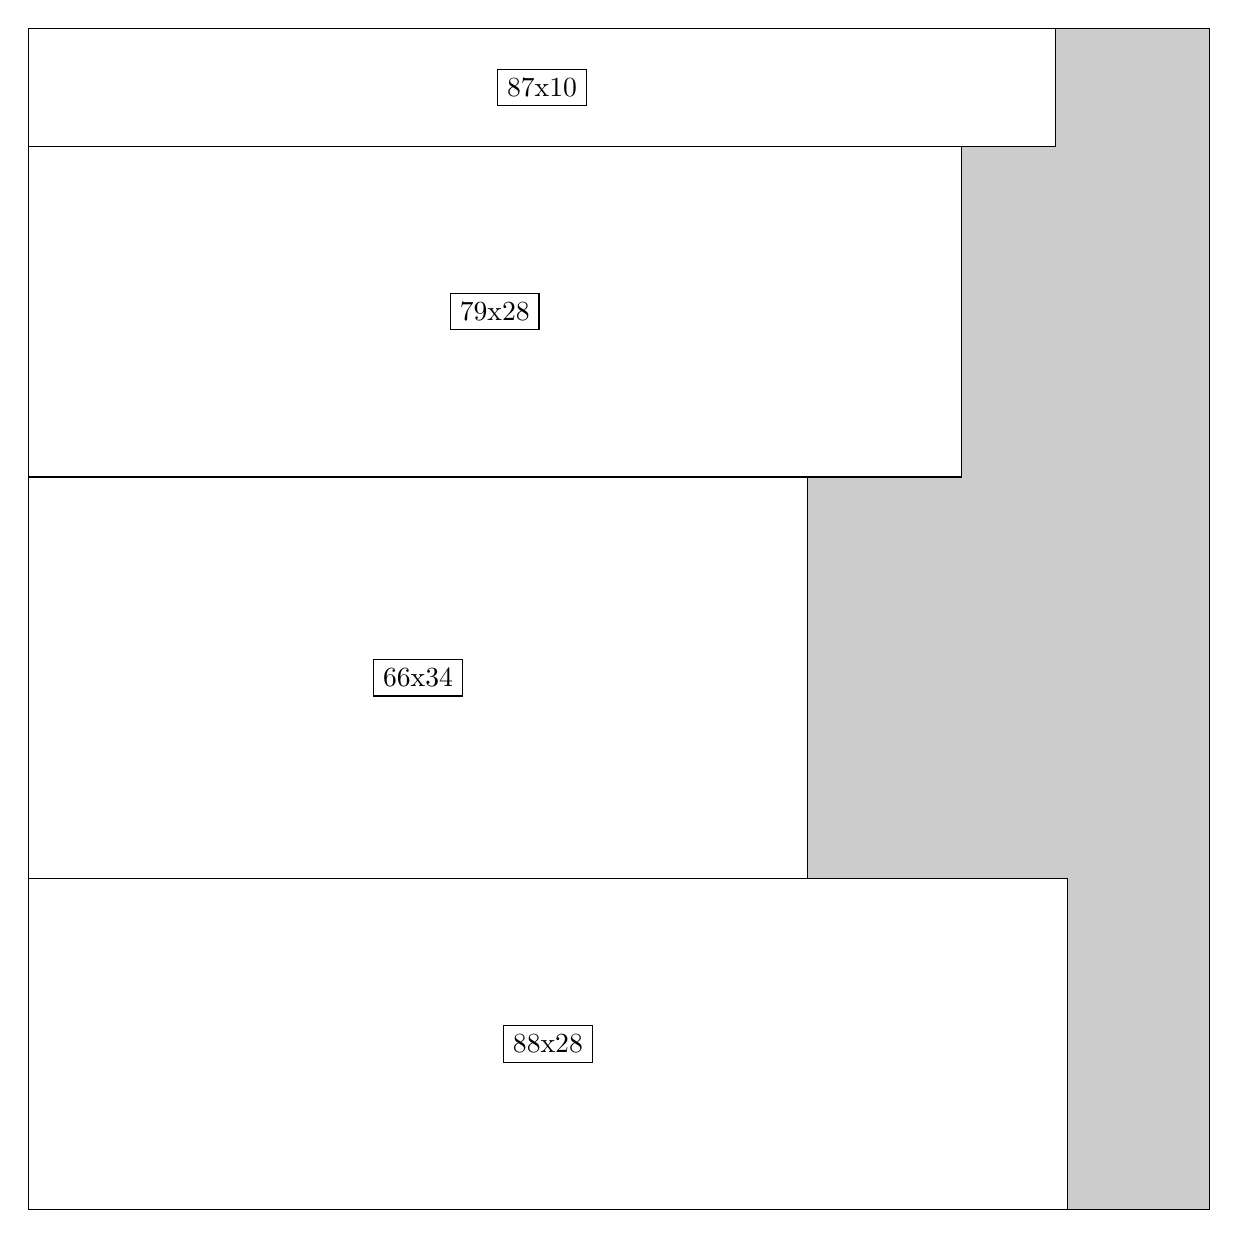
\begin{tikzpicture}[shorten >=1pt,scale=1.0,every node/.style={scale=1.0},->]
\tikzstyle{vertex}=[circle,fill=black!25,minimum size=14pt,inner sep=0pt]
\filldraw[fill=gray!40!white, draw=black] (0,0) rectangle (15.0,15.0);
\foreach \name/\x/\y/\w/\h in {87x10/0.0/13.5/13.049999999999999/1.5,88x28/0.0/0.0/13.2/4.2,66x34/0.0/4.2/9.9/5.1,79x28/0.0/9.299999999999999/11.85/4.2}
\filldraw[fill=white!40!white, draw=black] (\x,\y) rectangle node[draw] (\name) {\name} ++(\w,\h);
\end{tikzpicture}


w =87 , h =10 , x =0 , y =90 , v =870
\par
w =88 , h =28 , x =0 , y =0 , v =2464
\par
w =66 , h =34 , x =0 , y =28 , v =2244
\par
w =79 , h =28 , x =0 , y =62 , v =2212
\par
\newpage


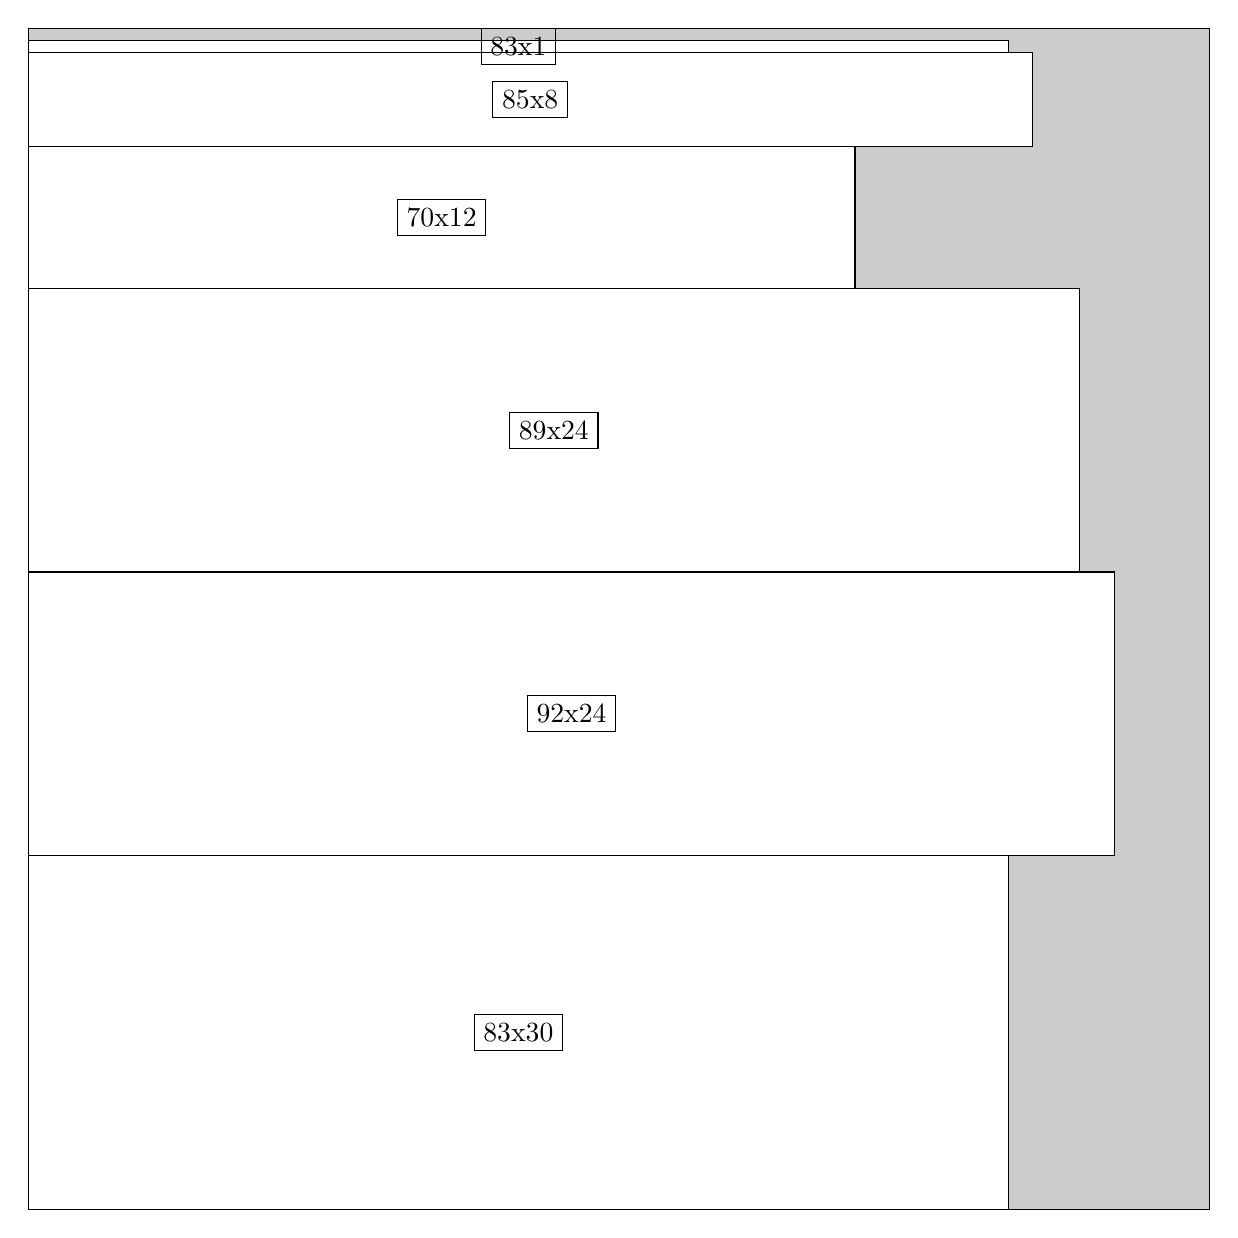
\begin{tikzpicture}[shorten >=1pt,scale=1.0,every node/.style={scale=1.0},->]
\tikzstyle{vertex}=[circle,fill=black!25,minimum size=14pt,inner sep=0pt]
\filldraw[fill=gray!40!white, draw=black] (0,0) rectangle (15.0,15.0);
\foreach \name/\x/\y/\w/\h in {83x30/0.0/0.0/12.45/4.5,92x24/0.0/4.5/13.799999999999999/3.5999999999999996,89x24/0.0/8.1/13.35/3.5999999999999996,70x12/0.0/11.7/10.5/1.7999999999999998,85x8/0.0/13.5/12.75/1.2,83x1/0.0/14.7/12.45/0.15}
\filldraw[fill=white!40!white, draw=black] (\x,\y) rectangle node[draw] (\name) {\name} ++(\w,\h);
\end{tikzpicture}


w =83 , h =30 , x =0 , y =0 , v =2490
\par
w =92 , h =24 , x =0 , y =30 , v =2208
\par
w =89 , h =24 , x =0 , y =54 , v =2136
\par
w =70 , h =12 , x =0 , y =78 , v =840
\par
w =85 , h =8 , x =0 , y =90 , v =680
\par
w =83 , h =1 , x =0 , y =98 , v =83
\par
\newpage


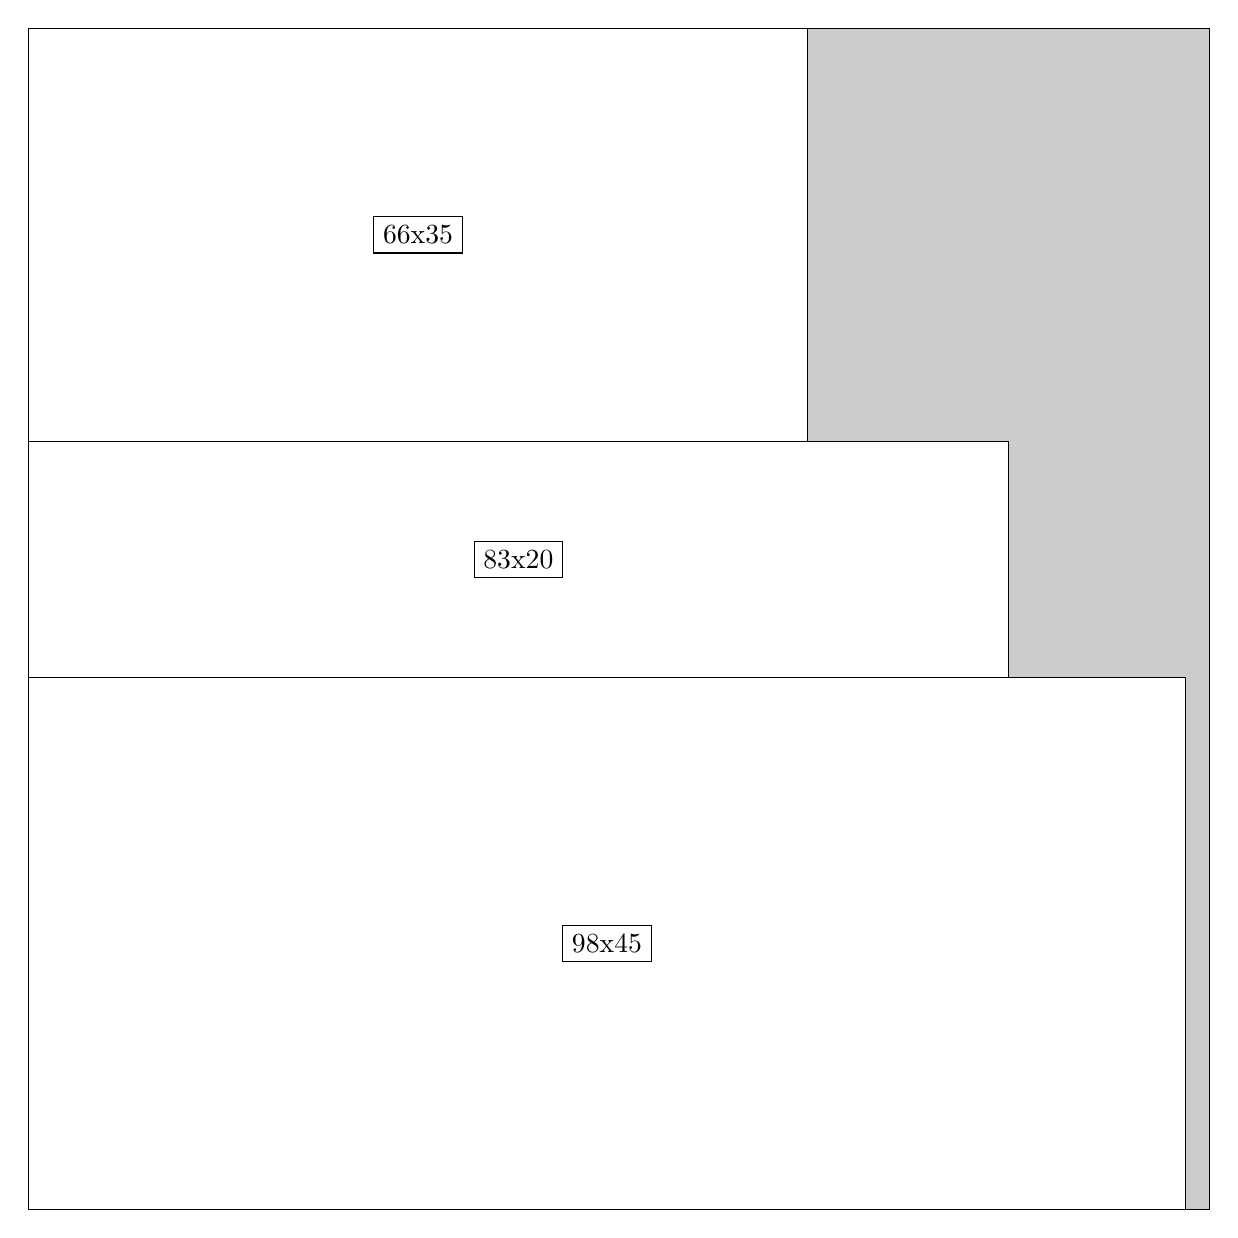
\begin{tikzpicture}[shorten >=1pt,scale=1.0,every node/.style={scale=1.0},->]
\tikzstyle{vertex}=[circle,fill=black!25,minimum size=14pt,inner sep=0pt]
\filldraw[fill=gray!40!white, draw=black] (0,0) rectangle (15.0,15.0);
\foreach \name/\x/\y/\w/\h in {98x45/0.0/0.0/14.7/6.75,66x35/0.0/9.75/9.9/5.25,83x20/0.0/6.75/12.45/3.0}
\filldraw[fill=white!40!white, draw=black] (\x,\y) rectangle node[draw] (\name) {\name} ++(\w,\h);
\end{tikzpicture}


w =98 , h =45 , x =0 , y =0 , v =4410
\par
w =66 , h =35 , x =0 , y =65 , v =2310
\par
w =83 , h =20 , x =0 , y =45 , v =1660
\par
\newpage


\end{document}